\documentclass[12pt]{article}
\usepackage[utf8]{inputenc}
\usepackage[T1]{fontenc}
%\usepackage[portuguese]{babel}
%\usepackage{tipa}%for \textchi etc
\usepackage{ifpdf,newtxtext,newtxmath} 
\usepackage{ amsmath, amssymb }
\usepackage{xcolor}
\usepackage{graphicx}
\usepackage{pdfpages}
\usepackage{wrapfig}
\usepackage{array,graphicx,dcolumn,multirow,hevea,abstract,hanging,fancyhdr,float}
% change next 3 lines each issue
\newcommand{\jdate}{}
\topmargin=-.3in \oddsidemargin=.3in \evensidemargin=.3in \textheight=9in \textwidth=6in
\pagestyle{fancy} 
\fancyhead[L]{\protect\small \href{\jref}{\jhead}, \date{\today}}
\fancyhead[R]{\protect\small  A STUDY OF SUPERCONDUCTING CIRCUITS FOR QUANTUM COMPUTING} % replace with running head
\fancypagestyle{firstpage}{%
 \lhead{\protect\small \href{\jref}{\jhead} \date{\today}}
 \rhead{}
}
\usepackage[labelfont=sc,textfont=sf]{caption}
\usepackage[hyperfootnotes=false,breaklinks=true]{hyperref} % was dvipdfmx
% \usepackage[hyperfootnotes=false,breaklinks=true,linkbordercolor={1 1 1},citebordercolor={1 1 1}]{hyperref}
% \usepackage{natbib} % must come afer hyperfootnotes, use 2nd version for bibtex
% \setlength{\bibsep}{0pt}
\urlstyle{rm}
\usepackage[hyphenbreaks]{breakurl}
% DO NOT USE ADDITIONAL PACKAGES unless you make sure they work with Hevea.
% You may define new commands, but these may cause other troubles, so try to avoid it.

\usepackage[backend=bibtex,style=chem-angew,citestyle=numeric-comp]{biblatex}
\addbibresource{bibliografia.bib}
% FOR BIBTEX USERS (Bibtex is not recommended, but we can use it):
% \usepackage{natbib} % must come afer hypperref
% in references: \bibliographystyle{apalike3} \setlength{\bibsep}{0pt} \bibliography{WHATEVER}
% download http://journal.sjdm.org/apalike3.bst
\usepackage{booktabs} % \toprule \midrule \bottomrule \cmidrule(lr){a-b}
% define centered and ragged columns:
\newcolumntype{L}[1]{>{\raggedright\arraybackslash }p{#1}} % can use m{}
\newcolumntype{C}[1]{>{\centering\arraybackslash }p{#1}}
\newcolumntype{R}[1]{>{\raggedleft\arraybackslash }p{#1}}
\newcolumntype{d}[1]{D{.}{.}{#1}} % d{3.2} for 3 places on l, 2 on r
\newcommand{\mc}{\multicolumn}
\setlength\tabcolsep{1mm}
\setlength\columnsep{5mm}
\setlength\abovecaptionskip{1ex}
\setlength\belowcaptionskip{.5ex}
\setlength\belowbottomsep{.3ex}
\setlength\lightrulewidth{.04em}
\renewcommand\arraystretch{1.2}
\renewcommand{\topfraction}{1}
\renewcommand{\textfraction}{0}
\renewcommand{\floatpagefraction}{.9}
% \renewcommand{\baselinestretch}{1.00} \large\normalsize % for fixing spaces
\widowpenalty=1000
\clubpenalty=1000
\setlength{\parskip}{0ex}
\let\tempone\itemize
\let\temptwo\enditemize
\let\tempthree\enumerate
\let\tempfour\endenumerate
\renewenvironment{itemize}{\tempone\setlength{\itemsep}{0pt}}{\temptwo}
\renewenvironment{enumerate}{\tempthree\setlength{\itemsep}{0pt}}{\tempfour}

\numberwithin{equation}{subsection}

\usepackage{enumerate}
%%%%%%%%%%%%%%%%%%%%%%%%%%%%%%%%%%%%%%%%%%%%%%%%%%%%%%%%%%%%%%%%%%%%%
% Create a new command for the horizontal rule in the document which allows thickness specification
\makeatletter
\def\vhrulefill#1{\leavevmode\leaders\hrule\@height#1\hfill \kern\z@}
\makeatother
\parindent 1cm

 \renewcommand{\rmdefault}{phv} % Arial
 \renewcommand{\sfdefault}{phv} % Arial

%\title{Relatório PIBIC Daniel Benvenutti}
%\author{}

\thispagestyle{empty}

\newcommand\ask[1]{
{%\color{red}
%#1
}
}

\newcommand\page[1]{
{
%\color{blue}\paragraph{
%Page #1
%}\mbox{}\\
}
}

\date{} % leave empty
\input notebooks-preamble.tex
\begin{document} % goes here

\setcounter{page}{1} % start with first page
\thispagestyle{firstpage}

\begin{wrapfigure}[2]{l}{7cm}

\includegraphics[width=6cm]{logo-documentos.png}
\end{wrapfigure}



\noindent 
\begin{flushright}
\begin{scriptsize}
Francisco Rouxinol \\
Instituto de Física Gleb Watghin\\
Rua Sergio Buarque de Holanda, 777\\
13083-859, Campinas, SP \\
e-mail: rouxinol@unicamp.br\\
tel: +55(19)3521-5462\\
% \hspace{-0.5cm} 
\vhrulefill{1pt} \\ % 
\end{scriptsize}
\end{flushright}

% \singlespacing %Para um espaçamento simples
% \onehalfspacing %Para um espaçamento de 1,5
%\doublespacing %Para um espaçamento duplo 

% $ $\\


% \singlespacing %Para um espaçamento simples
% \large 
\begin{flushleft}

\textbf{Grande Área de conhecimento}: Ciências Exatas e da Terra\\
\textbf{Área de Conhecimento}:Física\\
\textbf{Subárea de Conhecimento}: Física da Matéria Condensada\\
\textbf{Aluno(a)}:Daniel G. Benvenutti RA: 169448\\
\textbf{Orientador}: Francisco Rouxinol\\
\textbf{Instituição}: Instituto de Física Gleb Wataghin, UNICAMP\\
\textbf{Áreas de enquadramento da proposta}: Pesquisa Básica\\
\textbf{Áreas de enquadramento CNPq}: Tecnologias Habilitadoras: Materiais Avançados e Nanotecnologia\\
% \begin{itemize} \setlength\itemsep{0em}
% \item Tecnologias estratégicas: Cibernética
% \item 
% \item Tecnologias de Produção: Comunicações 
% \end{itemize}
\textbf{Palavras chaves}: Eletrodinâmica Quântica, Informação e Computação Quântica, Circuitos Supercondutores\\
\end{flushleft}

\section*{A study of superconducting circuits for quantum computing}
\begin{htmlonly}
\href{\jref}{\jhead} \date{\today} pp.\
\end{htmlonly}
%  \singlespacing %Para um espaçamento simples



\abstract{\textbf{The project introduces the student to the hardware of a quantum computer (QCH), more specifically to the hardware based on superconducting circuits based on Josephson junctions. We will study some of the main superconductor circuits used in implementation of QCH like the transmon qubit and the co-planar cavity. using capacitors, inductors and Josephson junctions, we will develop the main elements of these systems, and study the effects that a non-linear component, the Josephson junction, brings them. We will also study the interaction of a microwave cavity with and artificial atom, the transmon, and comprehend how this interaction will alter the states of these systems. using non-Hamiltonian simulations, in the qutip package, we will study the dynamics of this system. At last, we will implement these circuits in the package qiskit metal, an IBM tool, to generate the superconducting quantum circuits using these designs.}}

%  \singlespacing %Para um espaçamento simples


\section{Introduction}
In MIT's computer physics conference of 1981 Feymann said:\cite{Feynman1982SimulatingComputers} "\textit{ . . . trying to find a computer simulation of physics seems to me to be an excellent program to follow out. . . . the real use of it would be with quantum mechanics. . . . Nature isn’t classical . . . and if you want to make a simulation of Nature, you’d better make it quantum mechanical, and by golly it’s a wonderful problem, because it doesn’t look so easy}."
 This citation describes one of the most revolutionary fields of research of modern physics, from computer science and engineering, promising to be able to solve a category of computational problems that a classical computer cannot \cite{Nielsen2010QuantumInformation}. 
The key to build such device lies in implementing and controlling quantum bits (qubits, a quantum mechanical two level system) in a scalable way. Many approaches were adopted in the creation of different qubit realizations, like Rydberg atoms, electron spins, photons or superconducting circuits based on the Josephson junction \cite{Clarke2008SuperconductingBits}. 

In particular, in the last years there was a great progress in the development of quantum circuits in small scale with many quantum bits (qubits)\cite{Arute2019QuantumProcessor}. However, a quantum computer tolerant to faults that exceeds the development of existing classical machines currently will require a network of thousands or even millions of qubits, much beyond the current technologies \cite{Huang2020SuperconductingReview}. In this manner, the robust knowledge of control techniques and measurement of quantum machines is essential to the understanding of these new technologies.
With these words in mind, this project of scientific initiation has as objective the \textbf{ study of control techniques, measurement of quantum states of a qubit made out of elements of superconducting circuits}. The project will involve the \textbf{ study of the theory of many devices and fundamental concepts of the quantum technologies, like the simulation and techniques of fabrication of these systems}.
\section{Superconductors: macroscopic quantum phenomena\cite{gross2016applied} }
\subsection{The macroscopic quantum model}
\page{3,4 e 5}

People who are knowledgeable about quantum mechanics know that some quantum phenomena are quantized, manifest in discreet quantities. But it's interesting to notice that this isn't restricted to microscopic phenomena. Thanks to coherence effects the electrons in a superconductor are highly correlated. this can create quantization like in the magnetic flux of a superconducting loop with size orders of magnitude greater than an atom.



\subsubsection{Coherent phenomena in superconductivity}
The superconducting effect was studied many times by renowned researchers, but it was only really understood when Fritz London realised that it was but a quantum phenomenon manifesting in macroscopic scale. 

The macroscopic model of superconductivity assumes that there is a macroscopic wave function $\Psi(\textbf{r},t)$ describing the set of electrons. That in turn is justified by the BCS microscopic theory. Based on the idea that electrons feel an attractive force when near the Fermi level. Under a critical temperature the electrons go to a new quantum state where some electrons form Cooper pairs. These pairs don't have angular orbital momentum (estate \emph{s}) and therefore the Pauli exclusion principle requires that the spins be in a singleto ($||0,0\rangle$). In these pairs case the orbital state radius is much bigger (1nm até 1$\mu$m). With a great superposition in between the pairs. The bonding energy between these pairs depends on how many other pairs condensed and the center of mass is highly correlated. So much as that all remain in the same state with the same center of mass of movement.


The wave function of the movement of the mass center can be described as:
\begin{equation}
\Psi (\textbf{r} ,t)= \Psi_0 e^{i\theta(\textbf r,t)}= \Psi_0 e^{i\textbf{k}_s\cdot \textbf{r}-i\omega t } 
\end{equation}

This is valid for superfluids without charge such as the $^4He$, $^3He$ or the Bose-Einstein condensates.

\page{10}
\subsubsection{Finding a quantum equation for electromagnetism}

First we need to find \textbf{E} and \textbf{B} in potential terms. By Gauss's first law we know \textbf{B} can be written as:


\begin{equation}
    \mathbf{B} = \nabla \times \mathbf{A}
\end{equation}
\textbf{A} is a vectorial potential that we can use in the Faraday's law:
\begin{equation}
    \nabla \times \mathbf{E}+\frac{\partial \mathbf B}{\partial t}=\nabla \times (\mathbf{E}+\frac{\partial \mathbf A}{\partial t})=0 
\end{equation}
That implies:
\begin{equation}
   \mathbf E = \frac{\partial\mathbf A}{\partial t} -\nabla \phi
\end{equation}
Because the curl of a gradient of a scalar field $\phi$ is zero, we get the Lorentz law in the form:
\begin{equation}
    m \frac{d\mathbf v}{dt} = q[\mathbf E + (v \times \mathbf B)]
\end{equation}
Obtained in function of the potentials:
\begin{equation}
    m \frac{d\mathbf v}{dt} = -q[\nabla \phi + \frac{\partial A}{\partial t} -(\mathbf v \times (\nabla \times \mathbf A))]
\end{equation}

Using the chain rule:
\begin{equation}
\frac{d\mathbf A}{dt} = \frac{\partial \mathbf A}{\partial t} + (\mathbf v \cdot \nabla) \mathbf A
\end{equation}
 \page{11}
 
 We get:
 
\begin{equation}
    \frac {d}{dt} (m\mathbf{v} +q \mathbf A) =  -q [\nabla \phi + (\mathbf v \cdot \nabla)\mathbf A -(\mathbf v \times (\nabla \times \mathbf A))] 
\end{equation}
We can assume then (proof in reference\cite{gross2016applied}) that the canonical momentum is $\mathbf p = m \mathbf v +q \mathbf A$, where $m\mathbf v$ corresponds to the kinetical momentum and $q\mathbf A$ to the field momentum.
Then we obtain the law of Lorentz in the general form:
\begin{equation}
    \frac{d\mathbf p}{dt} = - \nabla \left\{ q\phi- \frac{q}{m} (\mathbf p \cdot \mathbf A) + \frac{q^2}{2m} \mathbf A \cdot \mathbf A)\right\}= - \nabla V
\end{equation}

Which shows that the potential isn't a function only of time and space but of the canonical momentum.

\page{12}
To find Schrödinger's equation we need the total energy ( to make the hamiltonian):
\begin{equation}
    E= E_{kin}+ E_{pot}  = \frac{\mathbf p \cdot \mathbf p}{2m}+\left\{ q\phi- \frac{q}{m} (\mathbf{p} \cdot \mathbf{A}) + \frac{q^2}{2m} \mathbf A \cdot \mathbf A)\right\} = \frac{1}{2m} (\mathbf{p} -q \mathbf{A})\cdot(\mathbf{p} -q \mathbf{A})+q\phi
    \label{eq:totalen}
\end{equation}
Then we substitute the energy and the momentum in the classical equation above (\ref{eq:totalen})
\begin{equation}
    E \rightarrow i\hbar \frac{\partial}{\partial t}
\end{equation}
    
\begin{equation}
    \mathbf{p}\rightarrow -i\hbar \nabla
\end{equation}
We obtain then the Schrödinger equation for a charged particle in an electromagnetic field:
\begin{equation}
    i\hbar \frac{\partial\mathbf \Psi}{\partial t}= \frac{1}{2m}\left( \frac{\hbar}{i}\nabla -q\mathbf A \right)^2 \mathbf \Psi + q \phi  \mathbf \Psi 
\end{equation}
That has a probability current:
\begin{equation}
    \mathbf J_\rho =\mathfrak R \left \{ \Psi^* \left(\frac{\hbar}{m}\nabla-\frac{q}{m} \mathbf A\right)\Psi      \right\} = \mathfrak R \left \{ \Psi^* \frac{\hat{ \mathbf p}}{m} \Psi      \right\}
\end{equation}

Supercurrent equation:
\begin{equation}
    \mathbf J_S = q^* n_S^*(\mathbf r,t) \left \{ \frac{\hbar}{m^*} \nabla\theta(\mathbf r, t) -\frac{q^*}{m^*} \mathbf A (\mathbf r, t)  \right \}
    \label{eq:supcur}
\end{equation}
Where $q^*$ is the superelectron charge and $n^*_S $ is the electron density (and the content inside the brackets is the speed $\mathbf v_s$)
\page{18}
\subsubsection{London Equations}
They are two equations by Fritz London that describe the behavior of superconductor on the basis of classical physics.

Assuming $n^*_S = cte$  in eq. \ref{eq:supcur}  (constant electron density). 


Using London's coefficient $\Lambda = \frac{m^*}{n^*_Sq^{*2}}$ the equation \ref{eq:supcur} becomes:

\begin{equation}
    \Lambda \mathbf J_S = - \left \{ \mathbf A(\mathbf r, t) -\frac{\hbar}{q^*}\nabla\theta (\mathbf r, t) \right \}
    \label{eq:supercurrent}
\end{equation}

\paragraph{Second London equation and the Meissner-Ochsenfeld effect\\}

\begin{figure}[h]
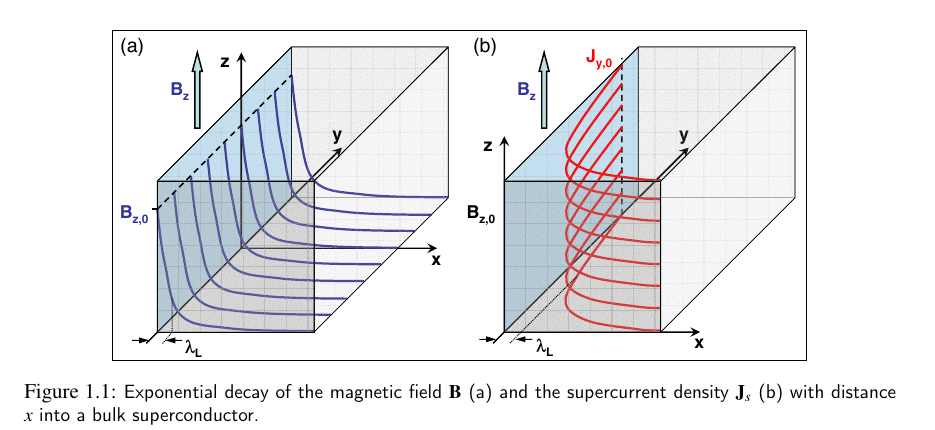
\includegraphics[scale=1.6]{images/second-london.png}
\caption{Adapted from: \cite{gross2016applied}}
\end{figure}[h]

With the curl of the expression obtained above we get the second London equation:

\begin{equation}
    \nabla \times (\Lambda \mathbf J_S) = -\nabla \times \mathbf A = -\mathbf B
\end{equation}

The Meissner-Ochsenfeld effect can be inferred from the equation obtained below: 
Taking the curl of the Maxwell equation:
\begin{equation}
    \nabla \times \nabla \times \mathbf B = \nabla \times \mu_0 \mathbf J_S
\end{equation}
Then the chain rule (left) and the second London equation (right):
\begin{equation}
    \nabla (\nabla \cdot  B) - \nabla^2 \mathbf B = - \frac{\mu_0}{\Lambda} \mathbf B 
\end{equation}
With $\nabla \cdot B =0$ we get:
\begin{equation}
    \nabla^2 \mathbf B = \frac{\mu_0}{\Lambda} \mathbf B = \frac{1}{\lambda_L^2} \mathbf B
\end{equation}
Where:
\begin{equation}
    \lambda_L \equiv \sqrt{\frac{m^*}{\mu_0n^*_Sq^{*2}}}
\end{equation}

This effect shows that we get a exponential decay inside a superconductor with an applied magnetic field where the characteristic decay length is the London penetration depth $\lambda_L$.

\paragraph{First London Equation and perfect conductivity\\}
To get the first London equation we take the derivative of eq. \ref{eq:supcur}
\begin{equation}
    \frac{\partial}{\partial t}  (\Lambda \mathbf J_S) = q^* n_S^*(\mathbf r,t) -\left \{\frac{\partial \mathbf A (\mathbf r, t)}{\partial t} -\frac{\hbar}{q^*} \nabla\frac{\partial \theta(\mathbf r, t)}{\partial t}   \right \}
    \label{eq:supcur}
\end{equation}

From the equation above, with:
\begin{equation}
    -\hbar \frac{\partial \theta}{\partial t}  = \frac{1}{2n^*_S} \Lambda \mathbf J^2_S + q^*\phi
    \label{eq:energy_phase}
\end{equation}
And with $ \mathbf E = - \partial \mathbf A /\partial t - \nabla \phi$ we can deduce the first London equation:
\begin{equation}
     \frac{\partial}{\partial t}  (\Lambda \mathbf J_S) = \mathbf E - \frac{1}{2n^*_Sq^*} \nabla (\frac{1}{2}\Lambda \mathbf J_S^2)
\label{eq:fstld}
\end{equation}
The second term in the right side of the London's equation can be neglected (because it's equivalent to the kinetic energy of the superelectrons) so we get:
\begin{equation}
     \frac{\partial}{\partial t}  (\Lambda \mathbf J_S) = \mathbf E 
\label{eq:fstldneglected}
\end{equation}
Where we can conclude that for a current constant in time the Electric field is zero and therefore we get a dissipation less current. $R=V/I=\int E d\mathbf r/I =0$ .

\page{19 e 20}
%\ask{Não consegui entender a esfera de london}
\subsection{Flux Quantization}
\page{24}
Analysis of the quantum mechanical properties of superconductors:

If you take a superconducting ring and apply a stationary current through a magnetic field. It will stay put through the zero resistance property. But it will also assume discreet ie quantized states as a consequence of it's quantumness. As a way that the wave function doesn't interfere destructively with itself. 
\begin{figure}[h]
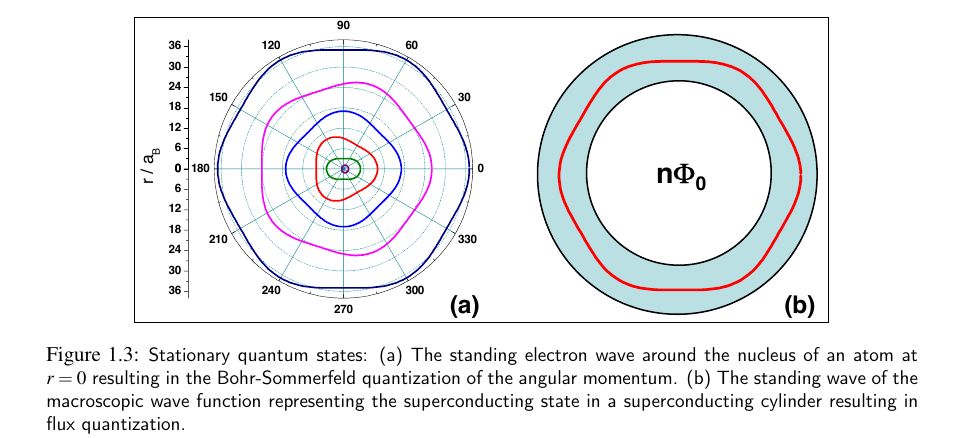
\includegraphics[scale=1.6]{images/flux-quantization.png}
\caption{Adapted from: \cite{gross2016applied}}
\end{figure}[h]
The values of the flux by this loop are multiples of the flux quantum:

\begin{equation}
    \mathbf{\Phi}^L_0 = \frac{h}{e} \approx 4\times 10^{-15} Vs
\end{equation}
But London derived this value without taking into account that the electrons form cooper pairs.
\page{25}
We then derive the quantization conditions from the macroscopic models for that we use equation \ref{eq:supercurrent} and integrate in a closed path:
\begin{equation}
    \oint (\Lambda \mathbf{J}_S) \cdot d\mathbf{l}  = -\oint \mathbf{A} \cdot d\mathbf{l} +\frac{\hbar}{q^*}\oint (\nabla \theta) \cdot d\mathbf{l}
    \label{eq:pathint}
\end{equation}
From stokes we get:
\begin{equation}
\oint \mathbf{A} \cdot d\mathbf{l} = \int_S(\nabla \times A)\cdot d\mathbf{s} = \int_S \mathbf{B}\cdot d\mathbf{s}
\end{equation}
The closed path integral of a gradient is always zero, but since the phase can actually be written as:
\begin{equation}
    \theta(\mathbf{r}, t) =     \theta_0(\mathbf{r}, t) +2\pi n
\end{equation}
The result of this path integral is $2\pi n$
%\ask{Eu não entendi o porquê de aquele limite que ele faz dá isso. Não iria cancelar o $2\pi n$ de $\theta_1$ com $\theta_2$?}

\page{26}

Equation \ref{eq:pathint} then becomes:
\begin{equation}
    \oint (\Lambda \mathbf{J}_S) \cdot d\mathbf{l} +\int_S \mathbf{B} \cdot d\mathbf{s} = \frac{\hbar}{q^*} 2\pi n=\frac{h}{q^*} n= \mathbf \Phi _0 n
    \label{eq:fluxoid}
    \end{equation}
and:
\begin{equation}
    \mathbf \Phi _0 = \frac{h}{|q^*|} =  \frac{h}{2e} 
\end{equation}
Consequences:
\begin{enumerate}

    \item The path defines a simply connected superconducting region: Here we just do the limit of the extremities $r_2\rightarrow r_1$. If the contour line has size zero then we just imply that $n=0$
    
    \item The path defines a multiply connected superconductor: Because of the hole inside the superconductor when you do the limit $r_1\rightarrow r_2$ they end up having a different phase. Which is $2\pi n$.
\end{enumerate}

\subsubsection{Flux and Fluxoid Quantizations}
The left side of the \ref{eq:fluxoid} equation is denoted \emph{fluxoid} and so it states the quantization of this fluxoid. 
Therefore the total flux in a multi-connected superconductor must have discreet values, even with an external magnetic field.
\paragraph{Flux quantization\\}
Assuming we have a superconducting ring with walls much thicker than the penetration depth $\lambda_L$ and a magnetic field much smaller than the critical field.
\page {27}
The magnetic field will pass inside the ring without penetrating the ring itself. On the ring's surface there will be screening supercurrents countering the incoming magnetic field. 

In case we cool down the superconductor with a magnetic field applied it can become trapped in it. But respecting the fluxonium quantization conditions though. By choosing somewhere inside the superconductor out of the penetration that where $\mathbf J_S\approx 0$ we get:
\begin{equation}
    \int_S \mathbf B \cdot d\mathbf s = n \Phi_0
\end{equation}
Which implies that quantization condition mentioned earlier.
\page{28}
\paragraph{Flux Trapping\\}
From the first London equation with $\partial\mathbf J_S/\partial t = 0 $, $\mathbf E=\partial\mathbf A/\partial t - \nabla \phi$ and $\nabla \phi = 0$ we get:

\begin{equation}
    \oint \mathbf E \cdot d\mathbf l = \frac{\partial}{\partial t} \oint \mathbf A \cdot d \mathbf l = -\frac{\partial}{\partial t} \int_S \mathbf B \cdot d \mathbf s = - \frac{\partial \phi}{\partial t}  
\end{equation}

Taking the path inside the superconductor so that $\mathbf E = 0$ we get $\partial \phi /\partial t = 0$. Which means the flux inside the cylinder.
stays constant. The supercurrents adjust themselves to maintain that.

\page{32}

\subsection{Josephson Effect}

This effect is observed if two superconductors are weakly connected by an electrical contact. Which can be a tunneling barriers, point contacts or regular conducting layers connecting them. 

The initial work by Josephson was SIS (superconductor insulator superconductor). For regular metals it's known that some electrons tunnel through the barrier with rate decaying exponentially to the length of the barrier. For superconductors there aren't regular electrons at Fermi level. So there will be \emph{no} tunneling unless we get a voltage smaller than twice the energy gap voltage $V<2\Delta /e$. For a greater voltage the Cooper pairs can be broken and then tunnel through the barrier.

About the possibility of a whole cooper pair tunneling. The probability is expected to be the square of the probability of a single electron $p_t\le 10^{-4}$ so $p_t^2$. Though Brian Josephson discovered that the probability is the same for a single electron. Because the tunneling of the pairs is coherent.

Also there is the \textbf{Josephson coupling energy} that works similar to the binding energy of a molecule. Because like the wave functions of the electrons of a hydrogen molecule overlap so does the wave functions of the two superconductors.

\begin{figure}[h]
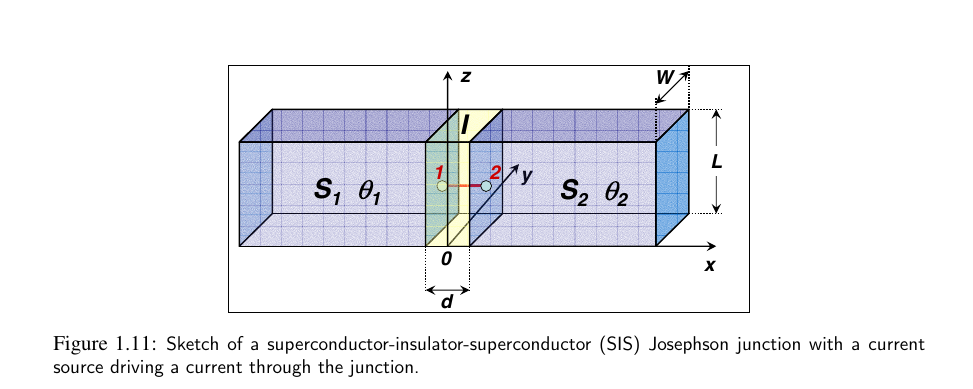
\includegraphics[scale=1.6]{images/superconductor-junction.png}
\caption{Adapted from: \cite{gross2016applied}}
\end{figure}[h]

\subsubsection{The Josephson Equations}
\page{34}
\paragraph{First Josephson Equation: current-phase relation\\}
We first assume that the supercurrent in the barrier is not great enough to affect $|\Psi|^2$ of either junction. Which is proportional to the cooper pair densities. However we expect the phase difference to play a role instead.

The supercurrent depends on the gauge invariant phase gradient:

\begin{equation}
    J_s(\mathbf r, t) = \frac{q^*n_s^*\hbar}{m^*} \left [ \nabla\theta(\mathbf r, t) - \frac{2\pi}{\Phi_0}\mathbf A (\mathbf r, t)  \right] = \frac{q^*n_s^*\hbar}{m^*} \gamma (\mathbf r, t)
\end{equation}

To simplify we assume:
\begin{enumerate}[I]
    \item The current density is homogeneous
    \item The phase gradient $\gamma$ is varying negligibly in the electrodes
    \item $\mathbf J_s$ is the same in the electrodes and the junction area (current conservation)
\end{enumerate}

Since $\gamma$ is invariant outside the junction region. For that reason we use the \textbf{gauge-invariant phase difference $\phi$}:
\begin{equation}
    \phi(\mathbf r, t) = \int^2_1\gamma (\mathbf r, t) = \int^2_1 \left( \nabla \theta - \frac{2\pi}{\Phi_0}\mathbf A \right ) \cdot d\mathbf l = \theta_2(\mathbf r, t) - \theta_1(\mathbf r, t)  +  \int^2_1  \frac{2\pi}{\Phi_0}\mathbf A(\mathbf r, t) \cdot d\mathbf l
\end{equation}
With an integration path along the current. That is, across the barrier from the superconductor with phase $\theta_1$ to $\theta_2$. And in the barrier.

$\mathbf J_s$ is a function only of $\phi$ thus $\mathbf J_s(\phi)$. But since the change of phase in a wave function is periodic. The current is also periodic in relation to the phase difference.
\begin{equation}
    \mathbf J_s(\phi) = \mathbf J_s(\phi+n2\pi)
\end{equation}
Also in case $\theta_1=\theta_2$ we get a zero current $\mathbf J_S (0+2n\pi)=0$
\page{35}

General case supercurrent on josephson junction:
\begin{equation}
    \mathbf J_S (\phi) = \mathbf J_C \sin \phi + \sum^{\inftyty}_{m=2} \mathbf J_m \sin(m\phi) \approx \mathbf J_C \sin (\phi)
    \label{eq:currphase}
\end{equation}
$\mathbf J_c$ is the critical or maximum Josephson current density determined by the coupling strength. The second term can be neglected in most cases.

The essence of this last equation can be summarized as:

\emph{The supercurrent density through a Josephson junction varies with the sine of the phase difference across the junction in the absence of scalar and vector potentials}
\page{36}

\paragraph{Second Josephson Equation\\}

We derivate the gauge invariant phase different:
\begin{equation}
    \frac{\partial \phi}{\partial t} = \frac{\partial \theta_1}{\partial t}+\frac{\partial \theta_2}{\partial t} - \frac{2\pi}{\Phi_0}\frac{\partial}{\partial t} \int_1^2 \mathbf A(\mathbf r, t) \cdot d \mathbf l
    \label{eq:der}
\end{equation}

Energy-phase relation:
\begin{equation}
    -\hbar \frac{\partial \theta}{\partial t} = \frac{1}{2n^*_s} \Lambda \mathbf J^2_S +q^*\phi
    \label{eq:enepha}
\end{equation}

Substituting \ref{eq:enepha} into \ref{eq:der}:
\begin{equation}
    \frac{\partial \phi}{\partial t} = \frac{1}{\hbar} \left( \frac{1}{2n^*_s} \Lambda  (\mathbf J^2_S(2)- \mathbf J^2_S(1)) +q^*(\phi(2)-\phi(1)) \right)- \frac{2\pi}{\Phi_0}\frac{\partial}{\partial t} \int_1^2 \mathbf A(\mathbf r, t) \cdot d \mathbf l
    \label{eq:der}
\end{equation}

We can assume $\mathbf J_S(2)= \mathbf J_S(1)$ because the current across the junction is continuous. Also $q^*/\hbar = 2\pi/\Phi_0$ resulting:
\begin{equation}
    \frac{\partial \phi}{\partial t} = \frac{2\pi}{\Phi_0} \int_1^2 -\left (\nabla \phi+ \frac{\partial\mathbf A}{\partial t} \right) \cdot d \mathbf l=  \frac{2\pi}{\Phi_0} \int_1^2 \mathbf E (\mathbf r, t) \cdot d \mathbf l
\label{eq:phase-efield}
\end{equation}
\page{37}
Which is the second Josephson equation. The integral is just the potential difference $V$ between the two superconductors 

With a constant voltage V we get:

\begin{equation}
    \phi(t) = \phi_0 +\frac{2\pi}{\Phi_0}V t
    \label{eq:cst-voltage}
\end{equation}
And we get a Josephson current:
\begin{equation}
    I_S(t) = I_C\sin\phi(t)
    \label{eq:josephson-current}
\end{equation}

The Josephson frequency is given by $\frac{\nu}{V}$:

\begin{equation}
    \frac{\nu}{V} = \frac{\frac{V}{\Phi_0}}{V}= \frac{1}{\Phi_0} \approx 483.6\frac{MHz}{\mu V}
\end{equation}

We can see by this that the Josephson junction is an oscillator controlled by voltage that can generate very high frequencies with a high sensitivity to the voltage input.

\subsubsection{Josephson Tunneling}
Now we use the wave matching method to find the maximum Josephson current density $\mathbf J_C$ on a tunneling barrier of thickness $d$.
\page{38}
We will solve the Schrödinger equation for each superconductor electrode and the barrier and then match the solutions at the boundaries to determine the missing coefficients.
The wave function for the electrodes is given by:

\begin{equation}
    J_s(\mathbf r, t) = q^*n_S(\mathbf r, t) \left [ \frac{\hbar}{m^*}\nabla\theta(\mathbf r, t) - \frac{q^*}{m^*}\mathbf A (\mathbf r, t)  \right] 
\end{equation}

The relationship between the current density and the phase is given by \ref{eq:currphase}, the current-phase relation.
We then assume a uniform tunneling barrier  and that the junction $Area=Length\cdot Width$  is small enough for the current density to be assumed uniform in the junction area (constant on y and Z).
Approximating the energy-phase relation \ref{eq:energy_phase}:

\begin{equation}
    -\hbar \frac{\partial \theta}{\partial t}  = \frac{1}{2n^*_S} \Lambda \mathbf J^2_S
\end{equation}
The term on the right hand corresponds to the kinetic energy of the superelectrons, so we write:

\begin{equation}
    -\hbar \frac{\partial \theta}{\partial t}  = -\frac{E_0}{\hbar}
\end{equation}
And the time dependent wave function is thus:


\begin{equation}
    \Psi(\mathbf r,t) = \Psi(\mathbf r) e^{-i(E_0/\hbar)t}
\end{equation}

Now to determine the wave function on the insulating barrier. The height of the potential of the barrier $V_0$ is assumed greater than $E_0$. Therefore the potential function $V(x)$ is a rectangular function with height $V_0$ and thickness $d$. We assume that the process is elastic (the superelectrons maintain their energy) so the time evolution is the same inside and outside the barrier. The Schrödinger equation is then:

\begin{equation}
    -\frac{\hbar^2}{2m^*} \nabla ^2\Psi(\mathbf r) = (E_0-V_0)\Psi(\mathbf r)
\end{equation}

Which is time independent because the potential $V_0$ is a constant. The solution is a simple sum of decaying and increasing exponentials:
\begin{equation}
    \Psi(x) = A\cosh(\kappa x)+B\sinh(\kappa x)
    \label{eq:insulwave}
\end{equation}
\begin{equation}
    \kappa = \sqrt{\frac{2m^*(V_0-E_0)}{\hbar^2}}
\end{equation}
The boundaries at $\pm d/2$ give:
\begin{equation}
    \Psi(-d/2)  = \sqrt{n^*_1} e^{i\theta_1}
\end{equation}
\begin{equation}
    \Psi(+d/2)  = \sqrt{n^*_2} e^{i\theta_2}
\end{equation}
Solving these with \ref{eq:insulwave} we get:
\begin{equation}
    A = \frac{ \sqrt{n^*_1} e^{i\theta_1}+ \sqrt{n^*_2} e^{i\theta_2}}{2\cosh(\kappa d/2}
\end{equation}

\begin{equation}
    B = \frac{ \sqrt{n^*_1} e^{i\theta_1}- \sqrt{n^*_2} e^{i\theta_2}}{2\sinh(\kappa d/2}
\end{equation}

With the supercurrent density:
\begin{equation}
    \mathbf J_S = \frac{q^*}{m^*} \mathfrak R \left \{ \Psi^*\left (\frac{\hbar}{i} \nabla    \right)\Psi \right \}
\end{equation}
And substituting \ref{eq:insulwave} we get now:

\begin{equation}
    \mathbf J_S = \frac{q^*}{m^*}\kappa \hbar  \mathfrak R \{ A^*B\}
\end{equation}
Substituting A and B will wield the supercurrent density equation \ref{eq:currphase} ($\phi=\theta_2-\theta_2$) and the maximum Josephson current density will be:
\begin{equation}
    \mathbf J_C =  -\frac{q^*}{m^*}\kappa \hbar \frac {\sqrt {n_1^*n_2^*}}{2\sinh(\kappa d/2) \cosh(\kappa d/2)} = -\frac{q^*\kappa \hbar}{m^*} \frac {\sqrt {n_1^*n_2^*}}{\sinh(\kappa d)}
\end{equation}

In practice the barrier height $V_0$ is of the order of a few eV and thus the decay $1/\kappa$ is less than a nanometer. The thickness of the barrier is a few nanometers therefore $\kappa d \gg 1$. In this case we can approximate $\sinh(2\kappa d)$ to $\frac{1}{2} e^{2\kappa d}$. Getting:
\begin{equation}
    \mathbf J_C = -\frac{q^*\kappa \hbar}{m^*} 2\sqrt {n_1^*n_2^*} e^{-2\kappa d}
\end{equation}

\begin{figure}[h]
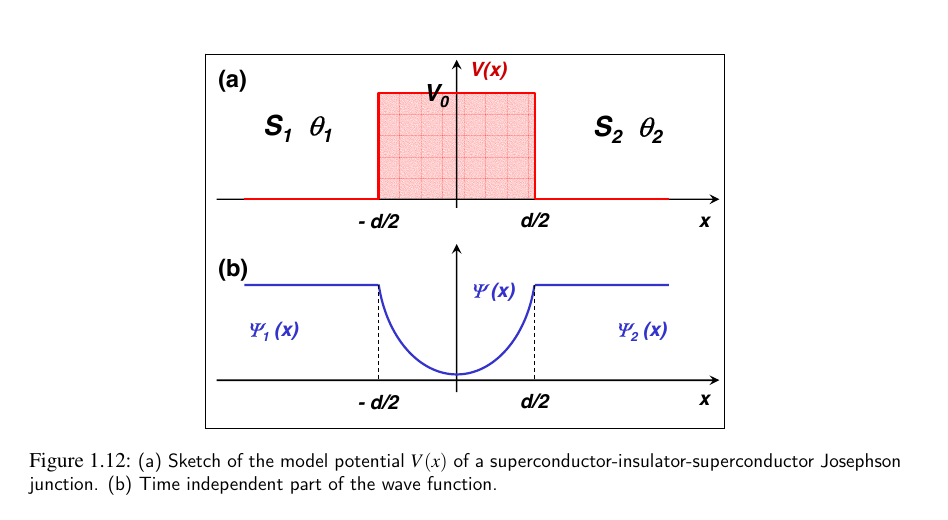
\includegraphics[scale=1.6]{images/potential-wavefunc.png}
\caption{Adapted from: \cite{gross2016applied}}
\end{figure}[h]

\section{Circuit QED: Superconducting Qubits coupled to microwave photons\cite{Girvin2015CircuitQS}}
\page{7}
\subsection{Quantum Electrical Circuits}
\subsubsection{Quantum LC oscillator}
A LC oscillator is composed of a capacitor and a inductor that oscillates just like a mass spring oscillator. With the charge accumulating on the capacitor and stopping current flow and then the flow starting again and accumulating flux on the inductor.
Given that the the supercurrent can flow without dissipation and the Coulomb interaction lifts the density fluctuations to optical frequencies we can approximate the LC oscilator as having a single degree of freedom of low energy. The uniform current flow on the inductor wire which builds charge only on the capacitor. This works well on a limit where the size of the wire is much smaller than the wavelength of light at the frequency of oscillation. 

\begin{figure}[h]
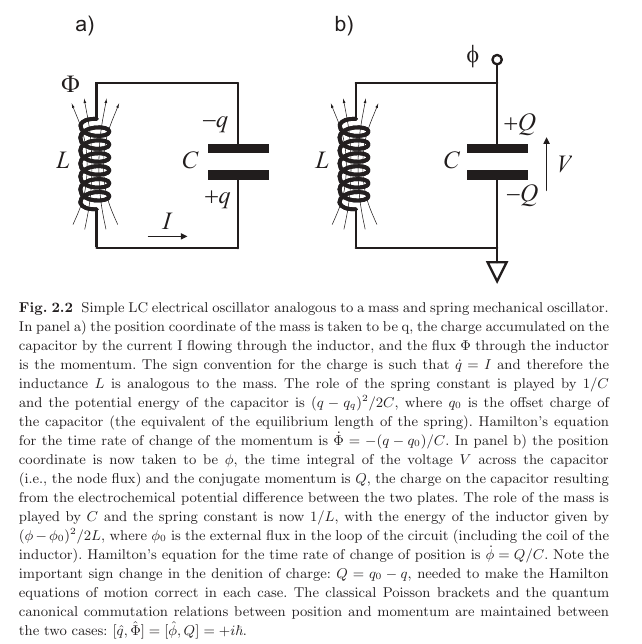
\includegraphics[scale=3]{images/9-lc-oscillator.png}
\caption{Adapted from: \cite{Girvin2015CircuitQS}}
\end{figure}[h]

The Lagrangian of the system is:
\begin{equation}
    \mathcal L = \frac{1}{2} LI^2 - \frac{1}{2}\frac{q^2}{C}
\end{equation}
\page{8}
The current is $I=\dot q$ and the momentum conjugate is the flux:
\begin{equation}
\frac{\partial \mathcal L}{\partial \dot q} = L\dot q = LI = \Phi
\end{equation}
Thus the Hamiltonian is:
\begin{equation}
    H= \Phi\dot q - \mathcal L = \frac{\Phi^2}{2L} + \frac{1}{2C} q^2
\end{equation}
The voltage on the capacitor is just $V=\dot \Phi$.

Quantizing the system we will get the non commuting opperators:
\begin{equation}
    [\hat \Phi , \hat q] = -i \hbar
\end{equation}
And the Hamiltonian can be written just like a regular harmonic oscillator:
\begin{equation}
    H = \hbar \frac{1}{\sqrt{LC}} (a^\dagger a + \frac{1}{2}) =  \hbar \omega (a^\dagger a + \frac{1}{2})
\end{equation}
\page{9}
And we can use the operators $a$ and $a^\dagger$ the same way as a regular Quantum Harmonic Oscillator. 
With the capacitance as the inverse of the spring constant $C = \frac{1}{k}$ and the inductance as the mass $L=m$. 

\begin{figure}[h]
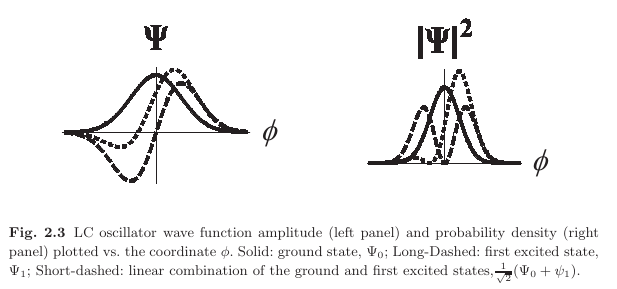
\includegraphics[scale=3]{images/14-wave-lc.png}
\caption{Adapted from: \cite{Girvin2015CircuitQS}}
\end{figure}[h]

\page{10}

Since we will use nonlinear inductors later it's more convenient to use the node flux:
\begin{equation}
    \Phi(t) = \int ^t d\tau V(\tau)
\end{equation}
Which implies $V(t)= \dot \Phi(t)$.

The potential and kinetic energy will be respectively:
\begin{equation}
    U=\frac{1}{2}C\dot\Phi^2
\end{equation}
\begin{equation}
    T = \frac{1}{2L} \Phi^2
\end{equation}
\page{11}
Also the Hamiltonian can be written as:
\begin{equation}
    H= \hbar\omega(a^\dagger a + \frac{1}{2})
\end{equation}
Just like the QHO.
The charge and flux operators are:
\begin{equation}
    \hat Q = - i Q_{ZPF} (a-a \dagger) = - i \sqrt{\frac{\hbar}{2Z}} (a-a \dagger)
\end{equation}
\begin{equation}
    \hat \phi = \Phi_{ZPF} (a+a^\dagger)=  \sqrt{\frac{\hbar Z}{2}}(a+a^\dagger)
\end{equation}

\page{12}
$Z=\sqrt{\frac{L}{C}}$ is the characteristic impedance of the oscillator.
And using the superconducting resistance quantum:
\begin{equation}
    R_Q=\frac{h}{(2e)^2} \approx 6453.20 \Omega
\end{equation}
we get a dimensionless characteristic impedance:
\begin{equation}
    z= Z/R_Q
\end{equation}
The characteristic charge and flux are thus:
\begin{equation}
    Q_{ZPF}= \sqrt{\frac{C\hbar \omega }{2}} = \sqrt{\frac{\hbar}{2Z}} =2e \sqrt{\frac{1}{4\pi z}}
\end{equation}
\begin{equation}
    \Phi_{ZPF}= \sqrt{\frac{L\hbar \omega }{2}} = \sqrt{\frac{\hbar Z}{2}}=\frac{h}{2e} \sqrt{\frac{z}{4\pi }}
\end{equation}
Where the uncertainty product is obeyed:
\begin{equation}
   Q_{ZPF}\Phi_{ZPF} = \frac{\hbar}{2} 
\end{equation}

The superconducting flux quantum above is given by 
\begin{equation}
    \Phi_0 = \frac{h}{2e} \approx 2.06783367 \mu V/GHz
\end{equation}
\page{13}
Which tells us that that the vacuum fluctuation of the voltage across a capacitor with 10GHz and $Z=100\Omega$ impedance in the resonator circuit is on the scale of $0.333\mu V$ which is interesting for being in the same scale of the routinely measured audio range. 
\ask{what audio range?}
\page{15}

 \paragraph{Driven LC Oscillators\\}
To drive an LC oscillator we need to use a current source ideally. Because a voltage source has zero impedance and would interrupt the oscillation (cause damping). In practice you use a resonator that will be driven by a capacitor or antenna that introduces a bit of damping. 

\begin{figure}[h]
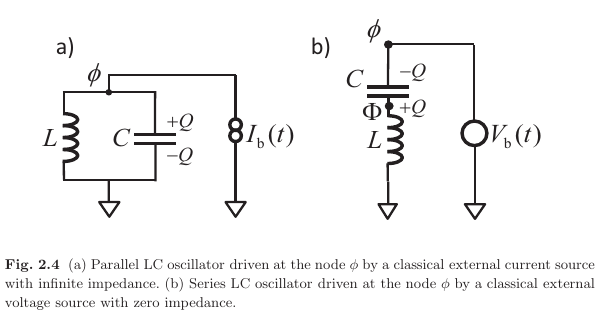
\includegraphics[scale=3]{images/15-driven-lc.png}
\caption{Adapted from: \cite{Girvin2015CircuitQS}}
\end{figure}[h]

The drive Lagrangian for the classical circuit would be:
\begin{equation}
    \mathcal L = \frac{1}{2} C\dot \phi ^2 - \frac{1}{2L} \phi^2+I_b(t)\phi
\end{equation}

The hamiltonian is:
 \begin{equation}
     H = \frac{Q^2}{2C} + \frac{\phi^2}{2L} - I_b(t)\phi
 \end{equation}
 You can also use a voltage source. But it has to be in series with the capacitor and inductor.
 \paragraph{Coherent States\\}
 We obtain a coherent state by driving a quantum system with a external classical force so that the ground state is mapped to it.
 \begin{equation}
     \Psi_0(\phi) \rightarrow \Psi_\Delta (\phi) = \Psi_0(\phi-\Delta)
 \end{equation}
 You can also displace a coherent state in momentum (charge).
 \page{17}
 It can be written too as:
 \begin{equation}
     \Psi_\Delta (\phi) =e^{-\Delta\frac{\partial}{\partial \phi}} \Psi_0 (\phi) = e^{-\frac{i}{\hbar}\Delta\hat Q} \Psi_0 (\phi) = e^{-\alpha (a-a^\dagger)} \Psi_0 (\phi) = U_\alpha \Psi_0 (\phi)
 \end{equation}
 Where $\alpha = \Delta Q_{ZPF}/\hbar = \Delta 2\Phi_{ZPF}$
 
 The state is thus using the Feynman disentangling theorem:
 \begin{equation}
     |\alpha \rangle = e^{-\frac{1}{2}|\alpha|^2} e^{\alpha a^\dagger} | 0 \rangle
 \end{equation}
 
 The coherent state has the following properties:
 \begin{equation}
     a|\alpha\rangle = \alpha | \alpha \rangle 
 \end{equation}
 But it's not an eigenstate of $a^\dagger$. The mean photon number is:
 \begin{equation}
     \langle \alpha|N|\alpha\rangle = |\alpha|^2 = \bar N 
 \end{equation}
 The phonon number distribuition is a Poisson:
 \begin{equation}
     P_n = |\langle n | \alpha \rangle |^2 = \frac{\bar N}{n!} e^{-\bar N}
 \end{equation}
 \page{18}
Time evolution:
\begin{equation}
    |\alpha(t)\rangle  =|e^{-i\omega t}\alpha(0)\rangle =e^{\frac{1}{2}|\alpha|^2} e^{\alpha e^{-i\omega t} a^\dagger} |0\rangle 
\end{equation}
This corresponds to a circular motion in phase space of the simple harmonic oscillator.
\begin{equation}
    \hat X = \frac{1}{2} [a+a^\dagger]
\end{equation}
\begin{equation}
    \hat Y = -i\frac{1}{2} [a-a^\dagger]
\end{equation}

\begin{equation}
    [X,Y] = \frac{i}{2}
\end{equation}
\begin{equation}
\langle \alpha |X | \alpha \rangle = \textrm{Real}\{ \alpha(t)\}
\end{equation}
\begin{equation}
\langle \alpha |Y| \alpha \rangle = \textrm{Imaginary}\{\alpha(t)\}
\end{equation}
\begin{equation}
\epsilon = X^2+ Y^2 = N+ \frac{1}{2}
\end{equation}
\page{19}
A coherent state is nothing more than a displaced vacuum state:
\begin{equation}
    |\alpha\rangle = U_\alpha |0\rangle
\end{equation}

Where $\alpha$ is the classical amplitude of the motion and if $|\alpha|\gg 1$ it dominates over the quantum fluctuations around the classical value. The $\alpha$ value is much greater compared to the deviation of the distribuition.

Writing the X quadrature amplitude as:
\begin{equation}
    X = \alpha + \Delta X
\end{equation}
The standard deviation operator above has the same properties as the sd of the position in vacuum state.

The number fluctuation is given bellow:
\begin{equation}
    \langle \alpha | \Delta N ^2|\alpha \rangle =     \langle \alpha |[2\alpha\Delta X + \Delta X ^2 + \Delta Y ^2 -1/2]^2 |\alpha \rangle = \bar N
\end{equation}

This means a coherent laser or beam is as classical as possible.

Fluctuations in the quadrature orthogonal to $\alpha$ cause uncertainty in a measurement of the coherent state. 
\ask{What does that mean? I don't understand}
If $\alpha \in \mathbb{R}$ and $|\alpha|\gg 1$. 
\begin{equation}
    \Delta \approx \frac{\Delta Y}{\alpha}
\end{equation}

\begin{equation}
\langle \alpha (\Delta \theta)^2|\alpha \rangle = \frac{1}{4N}
\end{equation}

\page{22}
Thus we arrive at the fundamental number-phase uncertainty:
\begin{equation}
\sqrt{     \langle \alpha | \Delta \theta ^2|\alpha\rangle}  \sqrt{     \langle \alpha | \Delta N ^2|\alpha\rangle} \ge  \frac{1}{2}
\end{equation}
From the equation of motion of the free oscillator we see that the quadrature of the amplitudes obey:
\begin{equation}
X(t) = \cos (\omega t) X(0)    +\sin (\omega t) Y(0)
\end{equation}
\begin{equation}
X(t) = \cos (\omega t) Y(0)    -\sin (\omega t) X(0)
\end{equation}
The sin and cos parts are quadrature of a quantum electrical signal and are canonically conjugate and thus can't be measured with perfect accuracy.
\subsubsection{Coupled LC Resonators}
Now we will quantize a pair of LC oscillators coupled by a capacitor. The Lagrangian will be:
\begin{equation}
    \mathcal{L} = \frac{1}{2} C_1\dot\Phi^2_1 +\frac{1}{2} C_2\dot\Phi^2_2+ \frac{1}{2} C_0 [\dot \Phi _1-\dot \Phi _2]^2- \frac{1}{2L_1}\Phi^2_1 - \frac{1}{2L_2}\Phi^2_2
\end{equation}
\page{23}
In matrix notation:
 
\begin{equation}
\mathcal{L} = \frac{1}{2}\dot \Phi \mathbf C\dot \Phi - \frac{1}{2}\Phi \mathbf L^{-1}\Phi 
\end{equation}

\begin{equation}
\mathbf C = \begin{pmatrix}
C_1+C_0 && -C_0 \\
-C_0 && C_2+C_0 \\
\end{pmatrix}
\end{equation}

\begin{equation}
\mathbf L^{-1} =
\begin{pmatrix}
1/L_1&& 0 \\
0 && 1/L_2\\
\end{pmatrix}
\end{equation}

\paragraph{Method I: Find the hamiltonian then diagonalize \\}

Canonical momenta:
\begin{equation}
    Q_i = \frac{\delta \mathcal L}{\delta \dot \Phi _i} = C_{ij} \dot \Phi_j
\end{equation}

With the Eistein notation for repeated indices.

The canonical momenta in terms of the inverse capacitance matrix:

\begin{equation}
    \dot \Phi = C^{-1} Q
\end{equation}
The Hamiltonian in the canonical form is now:
\begin{equation}
    H = \frac{1}{2} Q C^{-1} Q + \frac{1}{2} \Phi L^{-1} \Phi 
\end{equation}
\begin{equation}
    C^{-1} = \frac{1}{C_1C_2+C_0C_2+C_0C_2}
    \begin{pmatrix}
    C_2+C_0 & C_0\\
    C_0 & C_1+C_0
    \end{pmatrix}
    
\end{equation}

We now define two frequencies and a coupling constant:
\begin{equation}
    \omega_l^2 = \frac{1}{L_j} (C^{-1})_{jj}
\end{equation}
\begin{equation}
    \beta = \frac{C_0}{\sqrt{(C_1+C_0)(C_2+C_0)}}
\end{equation}
Then the inverse capacitance matrix becomes:
\begin{equation}
    C^{-1} = \begin{pmatrix}
    L_1 \omega_1^2 & \beta \sqrt{L_1 L_2} \omega_1\omega_2\\
    \beta \sqrt{L_1 L_2} \omega_1\omega_2 & L_2\omega_2
    \end{pmatrix}
\end{equation}

We can now write the Hamiltonian $H= H_0 +V$ in terms of two oscillators with masses $L_j$ coupled through their momenta. 
\begin{equation}
   H_0 = \frac{1}{2}L_1\omega_1^2Q^2_1 + \frac{1}{2L_1}\Phi^2_1+\frac{1}{2}L_2\omega_2^2Q^2_2 + \frac{1}{2L_2}\Phi^2_2
\end{equation}
\begin{equation}
    V = \beta \sqrt{L_1L_2}\omega_1\omega_2Q_1Q_2
\end{equation}
The quantization renders the canonical commutation relation:
\begin{equation}
    [\hat Q_i, \hat \Phi _j] = i\hbar \delta_{ij}
\end{equation}
Finally we get with the anihilation creation operators:

\begin{equation}
    H_0 = \sum^2_{j=0} \hbar \omega_j \left ( \hat a_j^\dagger\hat a_j + \frac{1}{2}\right )
\end{equation}
\begin{equation}
    V = - \beta \hbar \sqrt{\omega_1\omega_2})(\hat a _1 - \hat a _1^\dagger ) (\hat a _2 - \hat a _2^\dagger)
\end{equation}
Which can be diagonalized with the Bogoljubov transformation.
\ask{O que é essa transformação?}

\page{24}

\paragraph{Method II: Diagonalize the lagrangian, then the hamiltonian: \\}

The first method used the original coordinates and found thier canonical momenta and from there constructed the non-diagonal Hamiltonian. Here we will find the normal mode coordinates which diagonalize the Lagrangian. In terms of these, the Hamiltonian will be automatically diagonal. 

\page{25}

But the capacitance and inductance matrices do not commute. To solve that problem we make a similiarity transformation which maps $L^-1$ to the identity matrix. We then choose scaled coordinates:
\begin{equation}
    \psi_j = \frac{1}{\sqrt L_j} \Phi_j
\end{equation}
The Lagrangian now:
\begin{equation}
   \mathcal{L} = \frac{1}{2}\dot \psi_iA_{ij}\dot\psi_j-\frac{1}{2} \psi_i\delta_{ij}\psi_j 
\end{equation}
Where:
\begin{equation}
   A= \begin{pmatrix}
   \frac{1}{\Omega_1^2} && -\frac{\beta}{\Omega_1\Omega_2}\\
 -\frac{\beta}{\Omega_1\Omega_2}  && \frac{1}{\Omega_2^2} \\
    \end{pmatrix}
\end{equation}
And:
\begin{equation}
    \Omega^2_1 = \frac{1}{L_1(C_1+C_2)}
\end{equation}
\begin{equation}
    \Omega^2_2 = \frac{1}{L_2(C_2+C_0)}
\end{equation}
Letting S be the transformation matrix that diagonalizes A the normal modes and eigenvalues are then:
\begin{equation}
    \tilde \psi = S \psi 
\end{equation}
\begin{equation}
    \tilde A = S A S^T = \begin{pmatrix}
    \frac{1}{\Omega^2_1} & 0\\
    0 & \frac{1}{\Omega^2_2}
    \end{pmatrix}
\end{equation}

\page{26}

\subsubsection{Modes of Transmission Lines Resonators}

The topic of transmission lines will start with finite length transmission lines. That have discrete electromagnetic resonances, each an independent simple harmonic oscillator.
Then we will move to the semi-infinite ones. And see that they can act as a dissipative bath even without dissipative elements.
Our finite length line can be a coaxial cable or that which is relevant to the subject a 2D coplanar waveguide (CPW). Which is nothing but superconducting wire evaporated on an insulating substrate and with adjacent superconducting ground planes on the same surface. Figure \ref{fig:cpw}

\begin{figure}[h]
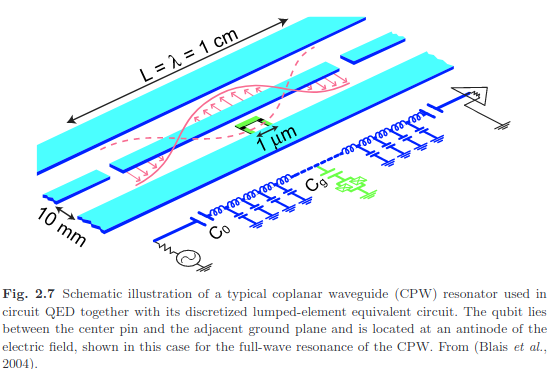
\includegraphics[scale=0.8]{images/26-cpw.png}
\caption{Adapted from: \cite{Girvin2015CircuitQS}}
\label{fig:cpw}
\end{figure}[h]
The discretized circuit is also show on figure \ref{fig:cpw}. For the innitial analysis the qubit and the capacitors $C_0$ will be ignored. Thus we can assume the current but not the voltage will vanish at the end of the transmission line.

\page{27}
It is convenient to define a new flux variable analogous to the above used but dependent on position. 
\begin{equation}
    \Phi(x,t) = \int^t_{-\infty} d\tau V(x,\tau)
\end{equation}
Where $V(x,t)= \partial_t\Phi(x,t)$ is the local voltage on the transmission line at position x and time t. The inductance and capacitance per unit length are \emph l and \emph c respectively.
Thus the inductance on a segment is $ l dx$, the voltage drop is $-dx \partial_x\partial_t\Phi(x,t)$ and the flux is $ -dx \partial _x \Phi(x,t)$ and the current is $I(x,t) = - \frac{1}{l} \partial_x \Phi(x,t)$.
A Lagrangian for a system of length L (not induction) is thus:

\begin{equation}
    \mathcal L_g = \int^L_0 dx \mathcal L(x,t) = \int ^L_0 dx \left [ \frac{c}{2}(\partial_t\Phi)^2 - \frac{1}{2l } (\partial _x\Phi)^2  \right]
    \label{eq:lag}
\end{equation}

The Euler-Lagrange equation for this Lagrangian is simply the wave equation:
\begin{equation}
v^2_p\partial^2_x\Phi - \partial ^2_t\Phi = 0
\label{eq:wave}
\end{equation}
The momentum conjugate to $\Phi(x)$ is simply the charge density
\begin{equation}
    q(x,t) = \frac{\delta \mathcal L_g}{\delta \partial_t \Phi} = c\partial_t \Phi = c V (x,t)
\end{equation}
And finally the Hamiltonian:
\begin{equation}
H = \int^L_0 dx \left \{ \frac{1}{2c} q^2 + \frac{1}{2l}(\partial_x\Phi )^2 \right \}
\end{equation}


Considering the classical normal mode solutions of the wave equation \ref{eq:wave} we get:
\begin{equation}
    \Phi (x,t) = e^{-i\omega t} \phi(x)
\end{equation}
We arrive at the Schrodinger like eigenvalue problem:
\begin{equation}
    -\partial^2_x\phi(x) = k^2\phi(x)
\end{equation}
Where $k=\omega/v_p$ and the mode wave velocity is $v_p = \frac{1}{\sqrt{le}}$.
The open-circuit model with zero current at the bondaries tells us that eigenfunctions have vanishing derivative at the boundaries. The normalization chosen is to keep the equation looking as close to those of a single harmonic oscillator.
\begin{equation}
    \phi_n(x) = \sqrt 2 \cos(k_n x )
\end{equation}
where $n \in \{0,1,2,3, ...\}$ and $k_n = \frac{n\pi}{L}$. 
\page{28}
Because the operator $\partial_x$ is self-adjoint for these boundary conditions and because the eigenvalues are non-degenerate the eigenfuction have the following helpful properties:
\begin{equation}
\int^L_0 dx \phi_n(x)\phi_m(x) = L \delta_{nm}    
\end{equation}

\begin{equation}
\int^L_0 dx [\partial_x\phi_n(x)][\partial_x\phi_m(x)] = Lk^2_n \delta_{nm}    
\end{equation}

From this it follows that the Lagrangian can be diagonalized using these spatial normal modes as basis(because they zero at non diagonal-equal indexes). The field parametrized becomes:

\begin{equation}
    \Phi (x,t) = \sum ^\infty _{n=0} \ksi_n(t)\phi_n(x)
\end{equation}
Where $\ksi_n$ are arbitrary functions of time (not necessarily complex exponentials).

Then we substitute this equation in the Lagrangian \ref{eq:lag} and using the properties
\begin{equation}
    \mathcal L_g = \frac{1}{2} Lc\sum^\infty_{n=0} [\partial_t \ksi_n]^2 - \omega^2_n \ksi^2_n
\end{equation}
We can see that each normal mode in the sum is an independent harmonic oscillator. The momentum conjugate to the normal mode amplitude is:
\begin{equation}
    q_n = \frac{\delta\mathcal L_g}{\delta\partial_t\ksi_n} = Lc\partial_t\ksi_n
\end{equation}
And the Hamiltonian is then:
\begin{equation}
  \hat  H = \frac{1}{2} \sum^\infty_{n=0} \left\{ \frac{1}{Lc}\omega_n^2\ksi_n^2 \right\}
\end{equation}

We can quantize this. The n=0 mode is just a free particle because the 'spring constant' is zero. In that case the momentum(charge) is constant and the position(flux) increases linearly with time. In most cases it can be ignored because the total charge is a constant and typically vanishes.

We end up with a set of independant normal modes with coordinate $\ksi_n$ and conjugate momentum $q_n$ which when quantized can be expressed in terms of mode raising and lowering operators:
\begin{equation}
   \hat \ksi_n = \sqrt{\frac{\hbar}{2\omega_nLc}}(\hat a_n+\hat a _n^\dagger)
\end{equation}

\begin{equation}
   \hat q_n = -i \sqrt{\frac{\hbar\omega_nLc}{2}}(\hat a_n-\hat a _n^\dagger)
\end{equation}
Where these ladder opperators obey:
\begin{equation}
[\hat a_n, \hat a_n^\dagger] = \delta_{nm}   
\end{equation}

\page{29}
If we couple a qubit to a ressonator at x, we need to express the flux and charge density operators at that point in terms of the normal operators:
\begin{equation}
   \hat \Phi (x) = \sum^\infty_n \phi_n(x)\hat\ksi_n 
\end{equation}
\begin{equation}
   \hat q(x) = \frac{1}{L}\sum^\infty_n \phi_n(x)\hat q_n 
\end{equation}
The voltage operator is just:
\begin{equation}
    \hat V (x) = \frac{1}{c}\hat q(x)
\end{equation}
The commutation relation is:
\begin{equation}
    [\hat q(x), \hat\Phi(x^\prime)] = -i\hbar \frac{1}{L} \sum^\infty_n \phi_n(x)\phi(x^\prime) = -i\hbar \delta(x^\prime - x)
\end{equation}
The Hamiltonian now becomes:
\begin{equation}
    \hat H = \int^L_0 dx \left \{ \frac{1}{2c}\hat q^2 + \frac{1}{2l} (\partial _x \hat \Phi)^2\right\}
\end{equation}
\ask{Eu não entendi o porque e o como dele chegar nessa equação de onda quantica}
\page{30}
Like the classical example of plucking a string we can coherently displace a linear combination of the normal modes.

Suppose we want to displace the resonator's degrees of freedom so that the local displacement obeys: 
\begin{equation}
    \langle \hat \Phi (x)\rangle = \Delta (x)
\end{equation}
Where $\Delta$ is a specified function. The analog of the displacement operator for the coherent states used before is just:
\begin{equation}
    U_\Delta = e^{-\frac{i}{\hbar}\int^L_0 dx \Delta(x)\hat q(x)}
\end{equation}

\page{44}
\subsection{Superconducting Qubits}
So far in studying the Cooper pair box a phenomenon has been ignored that is the build up of charge on the islands as current flows through the junction. Creating a Coulomb energy like a capacitor which makes it into a very good artificial atom.

There are many different kinds of superconducting qubits using the Josephson Junction such as the Cooper pair box based on charge, the flux qubit, the phase qubit and the fluxonium qubit. The works covering those are referenced in \cite{Girvin2015CircuitQS} chapter 4. These can be classified in a periodic table \ref{47-periodic} that shows their differences in the rations of energies and inductance of the Josephson junction.

\begin{figure}[h]
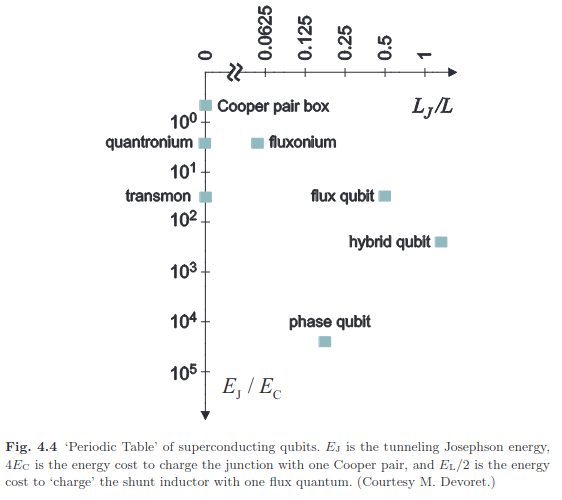
\includegraphics[scale=0.6]{images/47-periodic.png}
\caption{Adapted from: \cite{Girvin2015CircuitQS}}
\label{47-periodic}
\end{figure}[h]

\subsubsec{The Cooper pair box}
The cooper pair box (CPB) is topologically exceptional comparing to the other junctions given that it has no wire closing in the loop around the junction.The number of Cooper pairs transferred through the junction is a well defined integer. For this case the system is sensitive to stray electric field noise which is overcome by moving it down in the table \ref{47-periodic} towards the transmon. Where the tunneling energy ($E_J$) dominates the coulomb charging energy($E_c$).
The charging energy for a single electron is defined as:
\begin{equation}
    E_C = \frac{e^2}{2C_\Sigma}
\end{equation}
Where $C_\Sigma = C_J+C_g$ is the total capacitance between the islands. Illustrated in \ref{45-cpb}.

\begin{figure}[h]
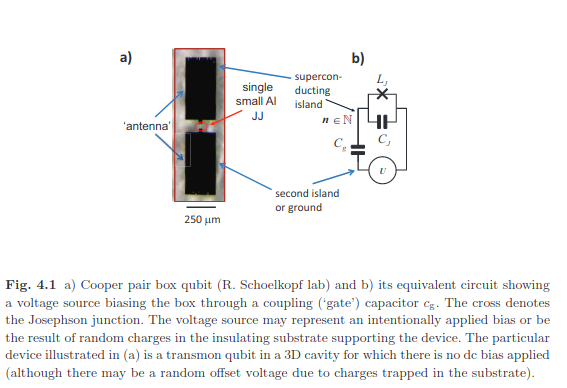
\includegraphics[scale=0.6]{images/45-cpb.png}
\caption{Adapted from: \cite{Girvin2015CircuitQS}}
\label{45-cpb}
\end{figure}[h]

The Coulomb energy to transfer a Cooper pair is four times that of an electron so we get the Coulomb energy operator:
\begin{equation}
    \hat U = 4E_C(\hat n - n_g)^2
\end{equation}
Where $n_g = -\frac{C_gV}{2e}$ is the dimensionless gate charge or offset charge that represents a break of degeneracy between the transfer of positive and negative charges caused by an external electric field or some junction asymmetry. It also fluctuates randomly (or intentionally). 
\page{48}
The phase difference of the junction $\varphi$ is compact. This means $|\varphi+2\pi \rangle = | \varphi \rangle$. The number operator is the conjugate angular momentum of $\varphi$ in the $\Varphi$ representation is given by:
\begin{equation}
    \hat n = +i\frac{d}{d\varphi}
\end{equation}
The Hamiltonian thus becomes:
\begin{equation}
    H = 4E_C(\hat n - n_g)^2 - E_J\cos\varphi
    \label{eq:cpb-h}
\end{equation}
In an analogy with a pendulum the charging energy($E_C$) is the inverse momentum of inertia and the Josephson energy ($E_J$) is the torque produced by gravity. For small amplitudes the classical pendulum is basically an harmonic oscillator. We can get a new approximated hamiltonian by expanding the cosine to second order:
\page{49}
\begin{equation}
    H \approx 4E_Cn^2 + \frac{1}{2} E_J \varphi^2
\end{equation}


From \ref{eq:phase-efield} and the $V(t)=\int^2_1E(\mathbf r, t) d\mathbf l=\frac{\partial \Phi(t)}{\partial t}$ relation
\begin{equation}
    \frac{\partial\varphi}{\partial t} = \frac{2\pi}{\Phi_0}\int^2_1\mathbf E (\mathbf r , t) \cdot d\mathbf l = \frac{2\pi}{\Phi_0} V_{1-2}(t) = \frac{2\pi}{\Phi_0} \frac{\partial\Phi}{\partial t} 
\end{equation}
Thus the phase angle is directly proportional to the flux in the junction:
\begin{equation}
    \varphi = \frac{2\pi}{\Phi_0} \Phi
\end{equation}
This means that each time the flux variable changes by one flux quantum ($\Phi_0$) the phase difference changes by $2\pi$. And the Hamiltonian becomes:

\begin{equation}
    H = \frac{1}{2C}Q^2 - E_J \cos \left (2\pi \frac{\Phi}{\Phi_0}\right)
\end{equation}
That approximated is:
\begin{equation}
    H = \frac{1}{2C}Q^2 + \cos 2\pi \frac{1}{2L_J}\Phi^2
\end{equation}
Where $L_J = \left(\frac{\hbar}{2e}\right)^2\frac{1}{E_J}$.
And approximated this way the CPB becomes a simple harmonic oscillator with resonant frequency(Josephson plasma frequency) given by
\begin{equation}
    \omega_J = \frac{1}{\sqrt{L_JC}} = \frac{1}{\hbar}\sqrt{8E_JE_C}
\end{equation}
\page{50}
For a general flux $\Phi$ we can define a differential inductance:
\begin{equation}
    L^{-1}(\Phi)=\frac{d^2H}{d\Phi^2} = E_J \left(\frac{2\pi}{\Phi_0}\right)\cos \left(2\pi\frac{\Phi}{\Phi_0}\right)
\end{equation}
Here we see that the Josephson junction acts as a non-linear inductor. This will make the energy levels of the CPB anharmonic like an atom. The reason we call such a device an artificial atom.

We can use this picture of a nonlinear inductor if the zero point fluctuations are small. But in general it's necessary to resort to numerical diagonalization of the CPB Hamiltonian.

For the full Hamiltonian in the ṕhase basis the Schrödinger eigenvalue equation is the Matthieu equation whose solutions are composed in terms of Matthieu functions.
\ask{O que são funções de Matthieu?}
The numerical diagonalization is more conveniently performed in the charge(number) basis where the Coulomb term is the diagonal and the Josephson term is tridiagonal ($\langle m\pm1|\cos\varphi |m\rangle = 1/2$. m are the eigenvalues of the operator $\hat n$ and are the labels of the eigenstates. The Hilbert state is truncated at some level $|m|=m_{max}$ that can be estimated from the zero point fluctuations of the charge:
\begin{equation}
    m_{max} \gg \sqrt{N}\frac{Q_{ZPF}}{2e} \approx \sqrt N \left(\frac {E_J}{32E_C}\right)^{1/8}
\end{equation}
The qubit spectrum is periodic in the offset charge $n_g$. So this means we can cancel the integer part of it by exchanging a integer number of Cooper pairs. 
\page{51}

The unitary transformation:
\begin{equation}
    U_\pm = e^{\pmi\varphi}
\end{equation}
Preserves the boundary conditions but shifts the angular momentum (transferred charge) by one unit
\begin{equation}
    U_\pm\hat nU_\pm^\dagger = \hat n \mp 1
\end{equation}
The pendulum analogy doesn't hold for the offset $n_g$. But we can consider it goes under an Aharanov-Bohm phase shift
\ask{What is this phase shift?}
as it circles a line of (fake) magnetic flux. The same way we substitute the canonical momentum for the mechanical momentum of a charged particle.
\begin{equation}
    \mathbf p \rightarrow \mathbf p - q\mathbf A(\mathbf r)
\end{equation}

For our pendulum turning on the z axis we use the angular momentum:
\begin{equation}
    L_z = (\mathbf r \times \mathbf p) \rightarrow  (\mathbf r \times \mathbf p)_z - q (\mathbf r \times \mathbf A)_z
\end{equation}
Considering a magnetic field that is null everywhere but this Aharanov-Bohm tube on the z axis the gauge we can chose is:
\begin{equation}
    \mathbf A(\mathbf r)  = \Phi_{AB} \frac{1}{2\pi r} \hat z \times \hat r
\end{equation}
\page{52}
Which has the correct total flux:
\begin{equation}
    \oint \mathbf A \cdot d\mathbf r = \Phi_{AB}
\end{equation}
For any loop with +1 winding number around $z$. The mechanical angular momentum is thus:
\begin{equation}
     (\mathbf r \times \mathbf p)_z -\frac{q}{2\pi}\Phi_{AB}  = \hbar \left( -i\frac{\partial}{\partial \varphi} - \frac{\Phi_{AB}}{\Phi_0}\right )
\end{equation}
Comparing it with the Hamiltonian \ref{eq:cpb-h} we see that the offset charge is equivalent fo the fake Aharonov-Bohm flux $n_g = \frac{\Phi}{\Phi_0}$

In the charge limit $E_C \gg E_J$ the states are nearly angular momentum states weakly perturbed by the Josephson coupling (gravitational force in the analogy). You can see how at this charge limit end the states in blue and red overlap when the charge is half-integer (figure \ref{51-cpb-spectru}). Also since the factor $E_C$ is big the excitation energies are influenced by a large extent by $n_g$ which is a noisy factor.


\begin{figure}[h]
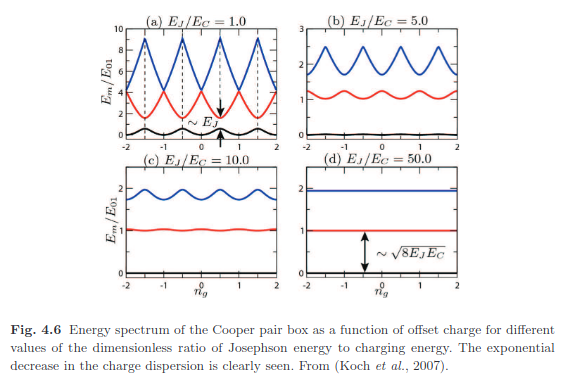
\includegraphics[scale=0.6]{images/51-cpb-spectrum.png}
\caption{Adapted from: \cite{Girvin2015CircuitQS}}
\label{51-cpb-spectrum}
\end{figure}[h]

On the other hand for the $E_J\ggE_C$ limit, the transmon limit. The pendulum motion are small amplitude harmonic oscillator like. Because now the gravitational force (out of the analogy $E_J$) is much more significant. The susceptibility to noise is much smaller too. Because for the fake Aharanov-Bohm flux to influence the pendulum, it has to complete an entire lap. And now the barrier that the system has to tunnel from $0$ to $2\pi$ is much greater and it's height proportional to $E_J$. And the particle 'mass' is also proportional to $1/E_C$.

\page{53}
Back to the language of wave function. We start with this unitary transformation that removes the offset charge term from the hamiltonian:
\begin{equation}
    U = e^{-i n_g\varphi}
\end{equation}

\begin{equation}
    U(\hat n - n_g)U^\dagger = \hat n
\end{equation}

An important detail is that the function does not obey periodic boundary conditions:
\begin{equation}
    U\Psi(\varphi + 2\pi) = e^{-i2\pi n_g} U\Psi(\varphi)
\end{equation}
But the Hamiltonian becomes independent of $n_g$:

\begin{equation}
UHU^\dagger = H = 4E_C\hat n ^2 - E_J \cos \varphi
\end{equation}
For a large $E_J/E_C$ the wave function is exponentially small at $\varphi = \pm \pi$. So we do not expect a large change in the spectrum due to the change in the boundary condition.
\ask{Por que?}

You can see how $n_g$ is less relevant to a junction under these conditions in \ref{51-cpb-spectrum} (d). Where a large $E_J/E_C$ factor has a flat constant energy level to a varying $n_g$. Although higher energy states can tunnel more easily through the barrier and so will have a higher charge dispersion.

\ask{Fiquei bem perdido nessa página em tudo depois da eq 4.27 do Girvin até antes da eq 4.31. Tem algo aqui que eu precise estudar a mais direitinho/colocar no relatório? Eu já pus as conclusões dessa parte no parágrafo anterior}
\page{54}
In this limit of large $E_J/E_C$ that the pendulum approaches an harmonic oscillator the anharmonicity defined by:
\begin{equation}
    A = \omega_{12}-\omega{01} \approx E_C
\end{equation}

goes to zero very slowly as the charging energy is reduced and can be kept above 100-200MHz which is adequate to prevent smooth nanosecond control pulses from taking the qubit to states out of the logical subspace (the two lower levels).

The anharmonicity can be estimated through perturbation theory by expanding the cosine above the second order:
\begin{equation}
   H \approx H_0+V = 4E_C\hat n^2 + \frac{1}{2} E_J \hat \varphi^2  + (-\frac{1}{24} E_J \hat \varphi ^4
\end{equation}

\page{55}
Also using $\hat \varphi = \varphi_{ZPF} (\hat a+ \hat a ^\dagger$ and $\varphi^2_{ZPF}= \sqrt{\frac{2E_C}{E_J}}$ the perturbation term is:
\begin{equation}
    V= -\frac{1}{24}E_J\hat \varphi^4 = -\frac{1}{12}E_C (\hat a + \hat a^\dagger)^4\approx - \frac{E_C}{2} (\hat a^\dagger\hat a^\dagger \hat a\hat a + 2 \hat a^\dagger \hat a)
\end{equation}
The second term in the final approximation renormalizes the harmonic oscillator frequency slightly down and the first will introduce this anharmonicity $-E_C$:
\begin{equation}
    A= \omega _{12} -\omega _{01} = \frac{E_C}{2} \langle 2| (\hat a^\dagger\hat a^\dagger \hat a\hat a)|2\rangle  =  \frac{E_C}{2} \sqrt{2} \cdot 1 \cdot 1 \cdot \sqrt 2 = -E_C
\end{equation}
\subsubsection{Inductively Shunted Qubits}
In the phase qubit the  the Josephson junction is shunted by a lumped element inductor. For the fluxonium a large inductance is needed. A value that is impossible to obtain with a coiled wire due to parasitic capacitances and the low value of the fine structure constant. Instead we use a long chain of Josephson junctions. The flux qubit uses only two making the shunting not linear.
%%%%%%
\page{56}

The great differences from a inductive shunted qubit to a regular CPB are the $\varphi$ and $\varphi + 2\pi$ are no longer equivalent because they differ in how much current flows through them. 
The charge variable now is also not continuous anymore because $\varphi$ is no longer a compact variable and the system doesn't obey periodic boundary values. So the energy store in the inductor diverges for large $|\varphi|$. Because of these new properties the $\varphi$ variable will be represented with a hat. The new hamiltonian is:
\begin{equation}
    H = 4E_C(\hat n -n_g)^2 - E_J\cos\hat\varphi + \frac{1}{2} E_L\hat \varphi^2
\end{equation}
Now with a continuous charge we can eliminate $n_g$ completely. And the spectrum will not depend on the static offset of the charge in any way for the transformed wave function $U\Psi$.
Since:
\begin{equation}
    E_L = \left ( \frac{\hbar}{2e}\right)^2\frac{1}{L} =  \left ( \frac{\Phi_0}{2\pi}\right)^2\frac{1}{L}
\end{equation}
If we take the limit $L \rightarrow \infty$ that implies $E_L \rightarrow 0$ the phase variable will no longer be compact but the term with the $E_L$ will no longer affect the Hamiltonian. Physically the high frequency oscillations of the qubit aren't affected but there is a continuous $k$ of states instead of discreet ones.

 $n_g$ doesn't affect the spectrum anymore because it only shifts the states $k \rightarrow k+n_g$ but all values of $k$ are allowed and the function is periodic $k\rightarrow k+1$.

\page{57}

If the inductive energy is non zero the Bloch theorem doesn't apply anymore. 
\ask{?}
The interplay between the quadratic term and the cosine from the Josephson term allows us to create many different potential wells shapes and generate an interesting spectra of qubits.

We can also control the externally applied flux which would be the inductive analog of the offset charge $n_g$ and will be called $\varphi_g$. The Hamiltonian is now:
\begin{equation}
    H = 4E_C(\hat n -n_g)^2 - E_J\cos\hat\varphi + \frac{1}{2} E_L(\hat \varphi - \varphi_g)^2
\end{equation}
We can translate these offsets using an unitary transformation:
\begin{equation}
    U=e^{i\varphi_g\hat n}e^{i\hat \varphi n_g}
\end{equation}
The hamiltonian then becomes:
\begin{equation}
    H = 4E_C(\hat n)^2 - E_J\cos(\hat\varphi+\varphi_g) + \frac{1}{2} E_L(\hat \varphi)^2
\end{equation}
We see now that the spectrum must be periodic in the offset flux.

To summarize the control knobs the experimentalist has are the variables: $E_J$, $E_C$, $E_L$ and $n_g$. Which allow us to create a rich variety of level structures.

The phase qubit operates around $E_J/E_C \approx 10^4$ which makes it very nearly an harmonic oscillator. 
To make it aharmonic a large flux bias is used on the inductor. But this also makes the energy level spacing small. 
\page{58}
So the junctions have a large area and a Josephson plasma frequency of $\omega_L = \sqrt {8E_JE_C}/h $ which is very high and around 50GHz.

\begin{figure}[h]
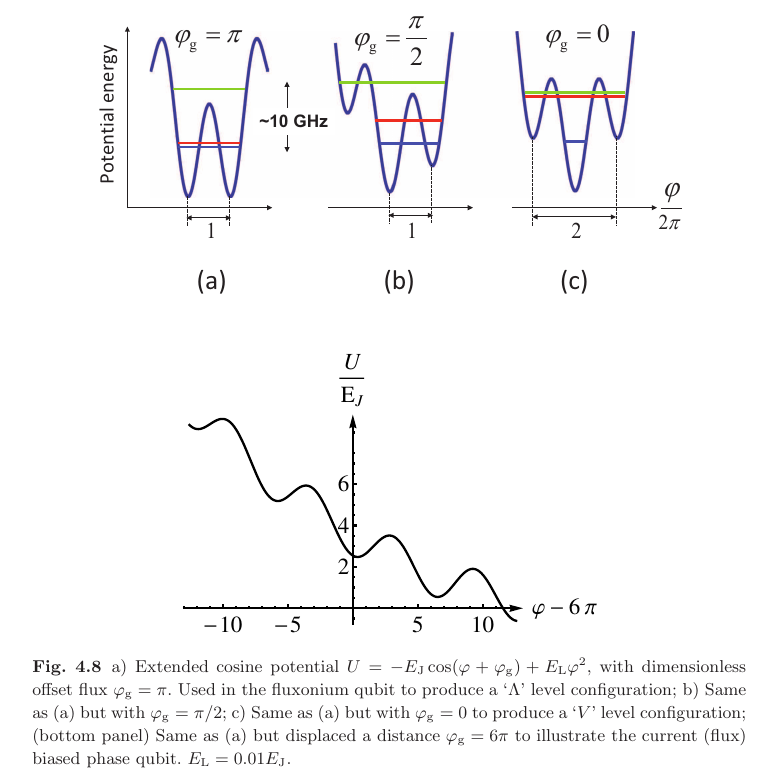
\includegraphics[scale=0.5]{images/58-fluxonium-wells.png}
\caption{Adapted from: \cite{Girvin2015CircuitQS}}
\label{58-fluxonium-wells}
\end{figure}[h]

\page{59}
In the Fluxonium qubit the large inductance is supplied by an array of Josephson junctions that generate a kinetic inductance. The anharmonicity can also be large.


In figure \ref{58-fluxonium-wells} (c) we can see the configuration of the potential well of the fluxonium for $\varphi_g = 0$. The ground state is supported by the middle valley and there are two excited states to the left and right. This is known as V configuration.
For \ref{58-fluxonium-wells} (a) there are two low states with a large gap to the next excited state. This is known as a '$Lambda$' configuration.
For \ref{58-fluxonium-wells} (b) finally the fluxonium varies smoothly between these two limits and does not have exponential sensitivity to external flux unlike the flux qubit.

\page{71}
\subsection{Introduction to Cavity and Circuit QED}
Cavity QED is about controlling the quantum fluctuations of the vacuum by creating a resonant cavity that supports discrete modes of an electromagnetic field.
One can alter the coupling of the atoms to their quantum environment by altering the frequencies and damping of the cavity. 
Because of the interaction of the photons in the cavity to the atoms one can enter a coherent superposition of these photons and the atom called \emph{polaritons}.
Using optical frequencies it's not possible to measure the state of the atom because the lifetime of spontaneous emission is of the order of nanoseconds. Though using microwaves the lifetime can be increased to around 30ms.

\begin{figure}[h]
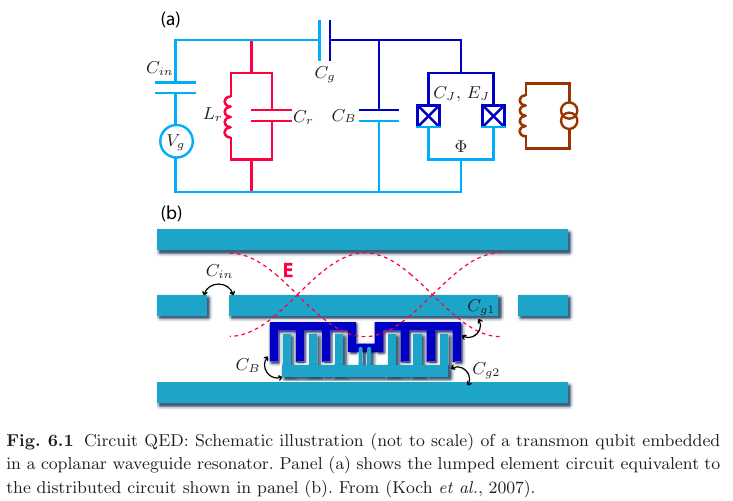
\includegraphics[scale=0.5]{images/73-circuit-qed.png}
\caption{Adapted from: \cite{Girvin2015CircuitQS}}
\label{73-circuit-qed}
\end{figure}[h]


Circuit QED uses superconducting qubits as artificial atoms coupled to microwave resonators (figure  \ref{73-circuit-qed}). Measuring the amplitude and the phase of microwaves transmitted (reflected) through the resonator.

\page{72}
Application of microwaves near the cavity frequency excites de cavity and performs a measurement while a microwave at the qubit transition frequency does not excite the cavity nor causes a measurement. These waves can be used to perform single qubit rotations.

In optical cQED a Frabry-Pérot cavity is used which is typically very large compared to optical wavelengths associated with atomic spectra. 

\page{73}
In circuit QED coupling can be arbitrarily strong because the antennae can be made as big as desired. The challenge is to obtain weak coupling to protect the qubit from the environmental noise by filtering it. The phyiscs of using a cabity to modify the coupling is that of a Purcell effect where a qubit is placed inside a cavity can have it's decay rate controlled by how far detuned or close from the cavity resonance. Which is useful for protecting superpositions in low detuning or for reseting the qubit with high detuning.
It can also be used to create single microwave photons on demand and enhance the transfer of quantum information from the artificial atom to the cavity photon.
One can view the Purcell effect
\ask{Eu preciso entender esse efeito? Ele menciona como se já fosse conhecido me parece com o efeito de um transformador numa impedancia pela descrição a seguir}
as the resonator performs an impedance transformation on the external dissipation of the environment to the qubit.

\page{74}
The coupling between the electric field in the cavity and the dipole moment of a single atom at $\mathbf r$ is:
\begin{equation}
    U=-\mathbf p \cdot \mathbf E(\mathbf r)
\end{equation}
We assume that only the cavity HO mode close to the atom transition frequency  is important.
The electric field at $\mathbf r$ can be written in terms of the mode polarization directing $\hat \epsilon$ and the zero point fluctuation $ E_{\textrm{ZPF}}$ at $\mathbf r$
\begin{equation}
\mathbf E = \hat \epsilon E_{\textrm{ZPF}}(\hat a+ \hat a^\dagger)
\end{equation}

Since the dipole moment operator connects to the ground and excited states of the two level atom the interaction Hamiltonian becomes:
\begin{equation}
    H_1 = \hbar g (\hat a+ \hat a^\dagger) \sigma_x
\end{equation}
Where $\sigma_x$ toggles the atom's states and g is the vacuum Rabi coupling given by the dipole matrix:
\begin{equation}
   \hbar g = \langle \Psi_1| \mathbf p \cdot \hat \epsilon |\Psi_0\rangle E_{\textrm{ZPF}} 
\end{equation}
The interaction Hamiltonian can be rewritten as:
\begin{equation}
    H_1 = \hbar g (\hat a\sigma_++ \hat a^\dagger\sigma_-)  +\hbar g (\hat a\sigma_-+ \hat a^\dagger\sigma_+)
    \label{eq:int-hamil}
\end{equation}
\page{75}
Where:
\begin{equation}
    \sigma_\pm = \frac{1}{2}(\sigma_x \pm i\sigma_y)
\end{equation}

We drop the second term of the equation \ref{eq:int-hamil} which is called doing a rotating wave approximation (RWA) because which is valid if the coupling is not very strong or if the detuning is so large  that no cavity mode is singled out. We can do this because the second term doesn't conserve the energy, a photon is created(destroyed) and the cavity also goes to the excited (ground) state and so is much less likely under those conditions.
The simplest approximation is using the Jaynes Cummings Hamiltonian with 
\begin{equation}
    H_0 = \hbar \omega_C\hat a^\dagger \hat a +\frac{\hbar \omega_{01}}{2} \omega_z
\end{equation}
\begin{equation}
    V = \hbar g (\hat a\sigma_++ \hat a^\dagger\sigma_-)
    \label{eq:vjaynes}
\end{equation}
The full hamiltonian is thus:
\begin{equation}
    H_0 = \hbar \omega_C\hat a^\dagger \hat a +\frac{\hbar \omega_{01}}{2} \omega_z + \hbar g (\hat a\sigma_++ \hat a^\dagger\sigma_-) + H_{\textrm{drive}}+ H_{\textrm{dampings}}
\end{equation}
Where the two hamiltonians in the end account for the external driving and damping which help control the states of the cavity.
\page{76/83}
Let the detuning between the qubit frequency and the cavity frequency be:
\begin{equation}
    \Delta = \omega_{01} - \omega_c
\end{equation}
\begin{figure}[h]
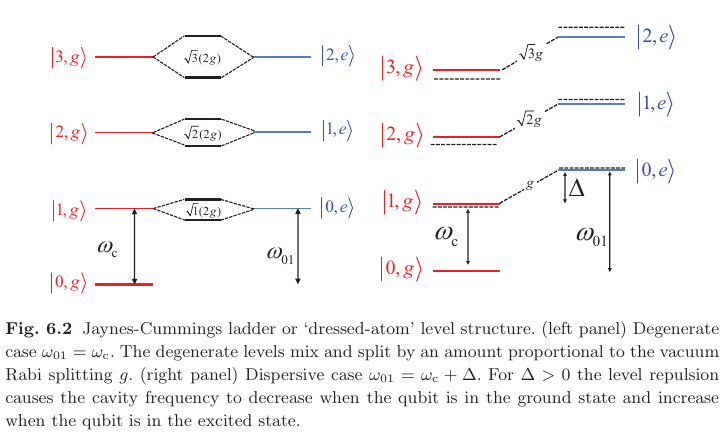
\includegraphics[scale=0.5]{images/76-coupling.png}
\caption{Adapted from: \cite{Girvin2015CircuitQS}}
\label{76-coupling}
\end{figure}[h]

Starting with $\Delta=0$ we see in figure \ref{76-coupling} (a) that there is a degeneracy of states such as $|1,g\rangle$ and $|0,e\rangle$. But there is also a break of this degeneracy lifted by the dipole coupling matrix element resulting in a $2g\sqrt{n+1}$ split. The split of $2g$ for the lowest pair is called vacuum Rabi splitting.

The energy eigenstates of the Hamiltonian $H_0 + V$ are given by:
\begin{equation}
    | \Psi _\pm\rangle = \frac{1}{\sqrt2} (|n+1,g\rangle \pm |n,e\rangle)
\end{equation}
And called bonding-anti-bonding combinations.

\page{77/84}

In the dispersive regime where $|\Delta| \gg g$ where the qubit is far detuned from the cavity. We will see that the diagonalization of the Hamiltonian to lowest order in $g$ leads to a second-order dispersive coupling.
\begin{equation}
    V_{\textrm{dispersive}} = \hbar \frac{g^2}{\Delta} \left [ \hat a ^\dagger \hat a + \frac{1}{2} \right ] \sigma_z
    \label{eq:dispersive}
\end{equation}
This coupling is quantum non-demolition (QND) with respect to photon number and qubit polarization since it commutes with both.
The dispersive coupling can be thought as either a shift in the cavity frequency which depends on the state of the qubit or as the ac-Stark light shift of the qubit frequency proportional to the number of photons in the cavity. 

The qubit-state-dependant shift of the cavity frequency leads to both changes in amplitude and phase of the reflected from or transmitted through the cavity and is the basis of the qubit readout in QND of the qubit state.

As required by a quantum measurement the photon shot noise in the cavity gradually dephases the qubit superposition as information is gained about $\sigma_z$. This is observed as a broadening spectroscopic line width of the qubit.

To derive the Hamiltonian in a dispersive regime (equation \ref{eq:dispersive}) we need to find a unitary transformation which removes the off diagonal term in equation \ref{eq:vjaynes}:
\begin{equation}
    U=e^{\hat \eta}
    \label{eq:dispersive-unitary}
\end{equation}
which is first order in g.

Using the Baker-Campbell-Hausdorff (BCH) expansion we have:
\begin{equation}
    \hat H = UHU^\dagger = H + [\hat \eta, H] + \frac{1}{2} [\hat \eta , [\hat \eta, H]]+ ...
\end{equation}
Substituting $H= H_0+V$ from perturbation theory and expanding the BCH only to the second term:
\begin{equation}
    \tilde H =H_0 + V+[\hat \eta, H_0]+[\hat \eta, V] + \frac{1}{2} [\hat \eta , [\hat \eta, H_0]]
\end{equation}

\page{78/85}

$\hat \eta$ Is chosen to satisfy:
\begin{equation}
  [\hat \eta, H_0] = -V  
  \label{eq:choseeta}
\end{equation}
We get then:
\begin{equation}
    \tilde H = H_0 + \frac{1}{2} [\hat \eta, V]
\end{equation}
It's easy to verify that eq. \ref{eq:choseeta} solution is
\begin{equation}
    \hat \eta = \frac{g}{\Delta} (\hat a \sigma_+ - \hat a^\dagger \sigma_-)
\end{equation}
This expansion is only valid for large enough detuning $g/\Delta \ll 1$. Otherwise the RWA expansion fails. The dispersive Hamiltonian is then:
\begin{equation}
    \tilde H = H_0 + \hbar \frac{g^2}{\Delta} \left( \hat a ^\dagger \hat a + \frac{1}{2} \right ) \sigma_z
    \label{eq:dispersiveH}
\end{equation}
Without drive or damping the Hamiltonian will commute with the excitation number that is the sum of the cavity excitation number and the qubit excitation number:
\begin{equation}
    \hat N _{\textrm{ex}} = \hat a \hat a ^\dagger + \frac{1+\sigma_z}{2}
\end{equation}
The solution then is of the form:
\begin{equation}
    \Psi^{(n+1)} = \alpha |n,e\rangle + \beta | n+1, g\rangle
\end{equation}
For which the $2\times 2$ eigenvalue problem becomes:
\begin{equation}
    H^{(n+1)}_{2\times 2} \begin{pmatrix}
    \alpha \\
    \beta
    \end{pmatrix}
    =E^{(n)}_\pm \begin{pmatrix}
    \alpha \\
    \beta
    \end{pmatrix}
\end{equation}

\page{79/86}

Where:
\begin{equation}
     H^{(n+1)}_{2\times 2}
     =\left(n+\frac{1}{2}\right) \hbar \omega_c + 
     \hbar\begin{pmatrix}
    \frac{\Delta}{2} & g\sqrt{n+1}\\
     g\sqrt{n+1}&\frac{-\Delta}{2} \\
    \end{pmatrix}
\end{equation}
The eigenvalues of these equation are:
\begin{equation}
    E^{(n)}_\pm =\left(n+\frac{1}{2}\right) \hbar \omega_c \pm \frac{\hbar}{2} \sqrt{\Delta ^2 + 4g^2 (n+1)}
\end{equation}
The eigenfunctions are:
\begin{equation}
    \Psi_+ = 
    \begin{pmatrix}
    \alpha_+ \\
    \beta_+
    \end{pmatrix}
    =\begin{pmatrix}
   \cos(\theta/2)\\
   \sin(\theta/2) 
    \end{pmatrix}
    
\end{equation}
\begin{equation}
    \Psi_- = 
    \begin{pmatrix}
    \alpha_- \\
    \beta_-
    \end{pmatrix}
    =\begin{pmatrix}
   -\sin(\theta/2)\\ 
   \cos(\theta/2)
    \end{pmatrix}
    
\end{equation}
Where:
\begin{equation}
    \theta = \tan^{-1} \left (   \frac{2g\sqrt{n+1}}{\Delta}  \right )
    \label{eq:theta-cav-atom}
\end{equation}
\paragraph{Dispersive limit ($g\ll \Delta$)} We can do a Taylor expansion of th energy eigenvalues to obtain:
\begin{equation}
    E^{(n)}_\pm =\left(n+\frac{1}{2}\right) \hbar \omega_c \pm \hbar \Delta \left [ \frac{1}{2} + \left(\frac{g}{\Delta}\right)^2 (n+1) - \left(\frac{g}{\Delta}\right)^4 (n+1)^2\right]
\end{equation}
We can reexpress it as an effective Hamiltonian:
\begin{equation}
    \tilde H =\left(\hat N_{ex}-\frac{1}{2}\right) \hbar \omega_c + \Sigma_z \hbar \Delta \left [ \frac{1}{2} + \left(\frac{g}{\Delta}\right)^2 (\hat N_{ex}) - \left(\frac{g}{\Delta}\right)^4 (\hat N_{ex})^2\right]
\end{equation}
Where $\Sigma_z = \pm 1$ is a spin label that smoothly connects to $\sigma_z$ in the limit $g\rightarrow 0 $ .

We can observe that the lowest term is like the dispersive Hamiltonian \label{eq:dispersiveH} and the next order term is some aharmonicity inherited from the qubit to the cavity (self-Kerr effect). 

\paragraph{$\Delta = 0$}  Here the uncoupled levels occur in degenerate pairs that are lifted by an amount proportional to $g$.

\begin{equation}
    E^{(n)}_\pm =\left(n+\frac{1}{2}\right) \hbar \omega_c \pm \hbar g \sqrt{n+1}
\end{equation}
The single excitation eigenstates are the polaritons mentioned before. Coherent superpositions of qubit and cavity excitations. The vacuum Rabi splitting can be observed spectroscopically. 
\page{80/87}
Because of the peculiar $\sqrt{n+1}$ and the excitation being half qubit half photon the polariton state is quite anharmonic which means we can treat one of the polariton states and the ground state as a two level system in the strong coupling limit. That also can be driven strongly without going up the excitation ladder and can be coherently flopped like a qubit.

Returning to the dispersive limit where the qubit is strongly detuned from the cavity. One polariton has primarily qubit character and the other primarily cavity character.

\page{81/88}

For the case of positive detuning it is $\Psi_=^{(n=0)}$ which is primarily qubit.
The rate of relaxation of this state is giving by the weighted averages of the bare qubit and cavity decay rates:

\begin{equation}
    \gamma_{\textrm{tot}} = \cos^2(\theta/2)\gamma + \sin^2(\theta/2)\kappa
\end{equation}

Where $\kappa$ is the cavity line width and $ \gamma$ is the atom line width. $\theta$ is from the equation \ref{eq:theta-cav-atom}.
For large detuning where $\sin^2(\theta/2)$ is small. The spontaneous emission of a photon via the cavity is very weak. We can say that the qubit must emit it's fluorescence photon into the cavity and pay the energy denominator price of a large detuning. Equivalently the cavity will filter out the vacuum noise at the qubit frequency which otherwise would cause fairly rapid spontaneous emition. 
\ask{this last sentence is for large detuning too, right?}
\page{82/89}

\ask{In this page he lists some other works and their acomplishments. Should I delve into it or leave it out?}

\page{83/90}
\subsubsection{Quantum control of Qubits in Cavities}
Suppose we apply a classical drive with a smooth envelope centered on the qubit transition frequency $\omega{01}$ to the cavity:
\begin{equation}
    V_d = \{v_R(t)\cos\omega_[01]t + v_R(t)\sin\omega_[01]t \} (\hat a^\dagger + \hat a)
\end{equation}

In the dispersive regime this drive is far removed from the cavity resonance and only weakly populates the cavity with virtual photons. The vacuum Rabi coupling term of the Jaynes-cummongs model in equation \ref{eq:vjaynes} can then cause coherent rotations of the qubit. This is most easily analyzed by applying the dispersive unitary transformation of equation \ref{eq:dispersive-unitary}. To lowest order in $g/\Delta$ we have the original rive on the cavity plus an effective drive directly on the qubit:
\begin{equation}
\tilde V_d \approx V_d+V{dq}
\end{equation}
Where:
\begin{equation}
    V_{dq} = [\eta, V_d] = \{ \lamba_R(t) \cos\omega_{01} t + \lambda_I(t)\sin\omega_{01} t   \} \sigma_x
\end{equation}
For large detuning ($\Delta \gg \kappa, \chi)$  the complex qubit drive amplitude given by
\begin{equation}
    \lambda_R(I) = v_{R(I)} (t) \frac{g}{\Delta}
\end{equation}
can be interpreted as the external drive filtered by the response function of the cavity. ( note that the filter factor is the same independent of the state of the qubit because $\Delta \gg \chi$.

We apply a unitary to take us into the rotating frame at the qubit transition frequency.
\begin{equation}
    U_{rot} = e^{\frac{i}{2} \omega_{01}t \sigma_z}
\end{equation}
And we are left with:
\begin{equation}
    H_{rot} = U_{rot} H U_{rot}^\dagger = \frac{\lambda_R(t)}{2} \sigma_x - \frac{\lambda_I(t)}{2} \sigma_y
\end{equation}
Thus we see that the cosine and sine drives produce rotations of the qubit around the $x$ and $y$ axes (in the rotation frame). Rotations in the z axis can be obtained in software by a combination of x and y rotations or in hardware by manipulating the qubit frequency to speed up or slow down the precession.
This gives us total control over the qubit state. % muahuahuahua

\page{84/91}

We have demonstrated that a single input wire to the cavity can be frequency multiplexed. 
A drive near the cavity frequency produces a dispersive measurement of the qubit state because the resonance frequency of the cavity and  hence the reflection coefficient depends on the state of the qubit. 

On the other hand a drive at the qubit frequency is so far detuned from the cavity frequency that reflection coefficient is independent of the state of the qubit and so almost no measurement (or measurement induced dephasing) occurs with coherent control pulses to rotate the qubit.

%Chapter 7
%The theory of quantum measurements has a long history starting with the founders of quantum mechanics torturing each other with the implications of various gedanken experiments and their interpretation. 
%;

%%%%%%%%%%%%%%%%%%%%%%%%%%%%%%%%%%%%%%%%%%%%%%%%%
%%%%%%%%%%%%%%%%%%%%%%%%%%%%%%%%%%%%%%%%%%%%%%%%%
\section{Qutip Jupyter notebook with a CNOT gate made of iSWAPs}
This section is a jupyter notebook that can be found on Github
\textcolor{blue}{\underline{\hyperlink{https://github.com/Danielgb23/ic-superconductor-qubit/blob/master/2-qubit-gates.ipynb}{(link)}}}
that simulates using Qutip a cavity plus two qubits system. That is controlled to do a series of one gate and two gates operations to obtain the equivalent of applying a CNOT gate plus some one qubit gate operations. Described with better details on the notebook:

References quoted in this notebook are Krantz's A quantum engineer’s guide to superconducting qubits \cite{2019krantz} and Wolfowicz's Pulse Techniques for Quantum Information Processing \cite{Wolfowicz2016PulseProcessing}.
\input notebook1-2-qubits.latex
%%%%%%%%%%%%%%%%%%%%%%%%%%%%%%%%%%%%%%%%
\section{Qutip Jupyter notebook to find the interaction factor between two qubits}
This section is a jupyter notebook that can be found on Github
\textcolor{blue}{\underline{\hyperlink{https://github.com/Danielgb23/ic-superconductor-qubit/blob/master/2-qubit-gates.ipynb }{(link)}}}

Here we simulate two qubits and vary the frequency of one of them to measure the amount of interaction it has with one another. In this case with a iSWAP gate like used before. Then we vary the time they interact and conduct a measurement from whose period of variation of the state transfer we can find $g$ the interaction factor. This is supposed to emulate a common process of calibration of this factor in a real quantum computer.

\input notebook2-finding-g.latex
%%%%%%%%%%%%%%%%%%%%%%%%%%%%%%%%%%%%%%%%%
\section{Qutip Jupyter notebook to simulate a measurement}
This section is a jupyter notebook that can be found on Github
\textcolor{blue}{\underline{\hyperlink{https://github.com/Danielgb23/ic-superconductor-qubit/blob/master/2-qubit-gates.ipynb}{(link)}}}
In the last notebook of the simulations we emulate the process of conducing a measurement through a cavity. For that we drive the cavity with a cosine wave and read the reflected/transmitted back wave with the $a$ operator expected value for the cavity. Different states of the qubit will result in waves with different frequency as explained further in the notebook.
\input notebook3-measurement.latex

\section{Building quantum chips with Qiskit Metal}
Using the tool from IBM, qiskit metal. I studied and modified two notebooks available from IBM tutorials:

\begin{itemize}

\item {\color{blue}\href{https://github.com/Qiskit/qiskit-metal/blob/main/tutorials/2%20From%20components%20to%20chip/C.%20My%20first%20full%20quantum%20chip%20design/2.21%20Design%20a%204%20qubit%20full%20chip.ipynb}{Design a 4 qubit full chip}}

%
\item {\color{blue}\href{https://qiskit.org/documentation/metal/circuit-examples/D.Qubit-couplers/31-TwoCrossmonsTunableCoupler.html}{Two Crossmons Tunable Coupler}}


\end{itemize}
Creating with these two tutorials a notebook for two transmon qubits coupled by a {\color{blue}\href{https://github.com/Danielgb23/ic-superconductor-qubit/blob/master/Design%20a%202%20qubit%20full%20chip.ipynb}{cavity}}
and another notebook for the transmons coupled by {\color{blue} \href{https://github.com/Danielgb23/ic-superconductor-qubit/blob/master/TwoTransmonsTunableCoupler.ipynb}{a coupler qubit}}. The first notebook was made by editing the "Design a 4 qubit full chip" tutorial to have only 2 qubits. So some parts where deleted and others rearranged in the code. The second notebook I made to generate the second chip is a mashup of both tutorials. I removed the crossmons which are another type of qubit and added two regular transmons in their place leaving the coupling qubit and rearranging it's position a little. Then using the knowledge of the first tutorial I added the launchpads and the connections between them and the transmons so the qubits can be controlled/measured.

\begin{figure}[h]
\centering
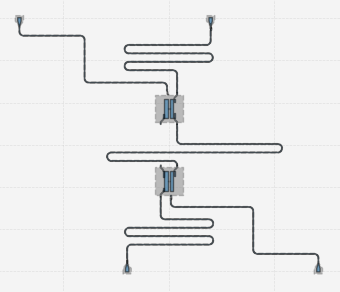
\includegraphics[scale=0.6]{images/metal-2qubits-cavity.png}
\caption{Chip of two transmon qubits coupled by a cavity}
\label{metal-cavity}
\end{figure}

\begin{figure}[h]
\centering
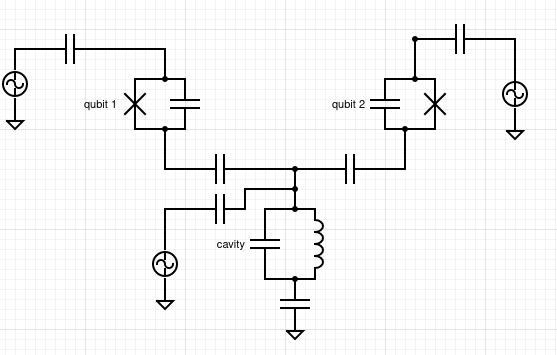
\includegraphics[scale=0.6]{images/metal-schematic-cavity.png}
\caption{Schematic of the chip of two transmon qubits coupled by a cavity}
\label{metal-schematic-cavity}
\end{figure}


\begin{figure}[h]
\centering
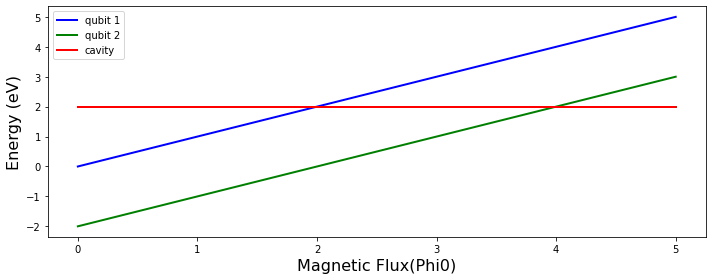
\includegraphics[width=\maxwidth,height=\maxheight,keepaspectratio]{images/metal-graph-cavity.png}
\caption{Illustrative graph of the energies of the qubits in function of the magnetic flux for two variable  qubits and a fixed cavity}
\label{metal-graph-cavity}
\end{figure}


The qubits coupled by the cavity (chip created in figure \ref{metal-cavity} and schematic in figure \ref{metal-schematic-cavity}). And will  change their energy according to the magnetic flux that is generated with a coil over the chip while the cavity doesn't change (figure \ref{metal-graph-cavity}). The qubits can be made to vary with the magnetic flux by having a double Josephson junction both in parallel. When the energy of the qubits is the same as the cavity they enter into a resonance that will allow us to use two qubit gates like the iSWAP. The energy of the qubits depends on many parameters such as the capacitance, the Josephson junction and the resistance in the junction. That way we can tune each qubit to have different behaviors.

\begin{figure}[h]
\centering
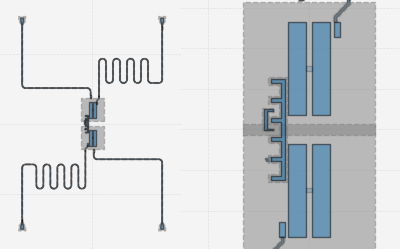
\includegraphics[scale=0.6]{images/metal-coupler.png}
\caption{Chip of two transmon qubits coupled by a third coupler qubit(with a close up to the right)}
\label{metal-coupler}
\end{figure}


\begin{figure}[h]
\centering
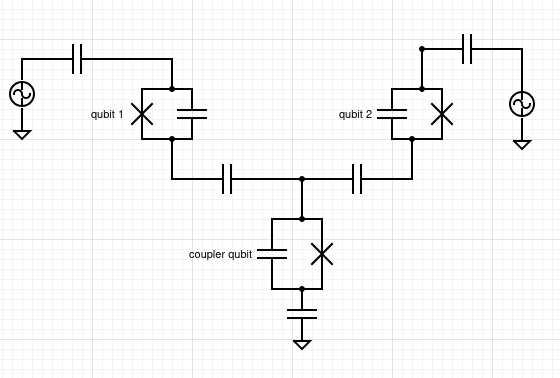
\includegraphics[scale=0.6]{images/metal-schematic-coupler.png}
\caption{Schematic of the chip of two transmon qubits coupled by a third coupler qubit}
\label{metal-schematic-coupler}
\end{figure}



\begin{figure}[h]
\centering
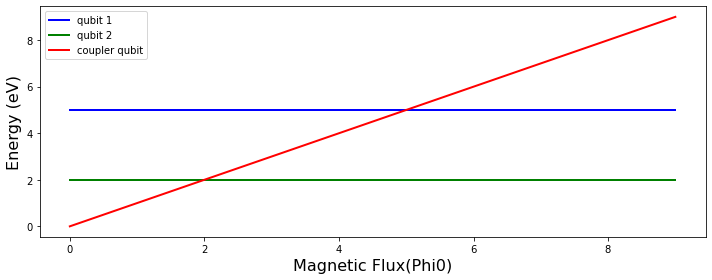
\includegraphics[width=\maxwidth,height=\maxheight,keepaspectratio]{images/metal-graph-coupler-qubit.png}
\caption{Illustrative graph of the energies of the qubits in function of the magnetic flux for two fixed qubits and a third variable coupler qubit}
\label{metal-graph-coupler}
\end{figure}



The qubits coupled by another qubit (figure \ref{metal-coupler} schematic in figure \ref{metal-schematic-coupler}) have a qubit between them that can have his energy adjusted by the magnetic flux. In that case we can bring the coupler qubit in and out of resonance with either qubit to do the 2 qubit gates like in figure \ref{metal-graph-coupler}. In our chips this might not make a lot of difference. But for multiple qubits this can make it easier to pick the qubits that we want to put into resonance with each other or not put.

\clearpage

\section{CST electromagnetic simulation of a quantum chip}
Here the circuit built in qiskit metal (figure \ref{metal-cavity}) will be simulated in electromagnetic simulators by numerical methods using the Maxwell equations for discreet regions of spaced named meshes. Getting numerical solutions to the electrical and magnetic fields for systems with complex geometries such as this one. The chosen simulator software is \textbf{CST} and the circuit used is exported from qiskit metal in the format GDS. 

The goal was finding the resonance frequency of the cavity between the two qubits. So it was edited in Klayout to cut out some parts of the circuit and leave only the relevant part in. Then it was imported in CST as a $1\mu m$ thick perfect electro conductor with a subtract of silicon under it (figure \ref{cst-component}). 


\begin{figure}[h]
\centering
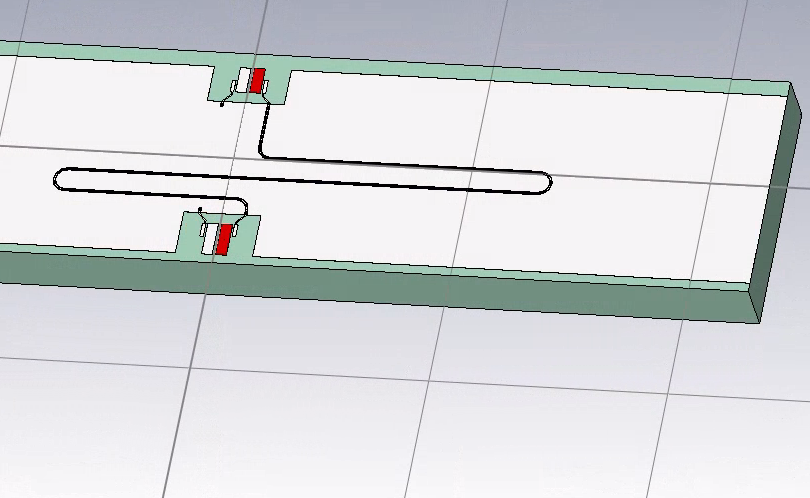
\includegraphics[width=\maxwidth,height=\maxheight,keepaspectratio]{images/cst-component.png}
\caption{3D model of the circuit for the simulation}
\label{cst-component}
\end{figure}

The signal input was placed at a plate of one transmon qubit and the output at the plate of the other qubit. And the simulation was run for many frequencies in the interval 0-20GHz. We can see the field monitor for 4GHz, figure \ref{cst-efield4}, and 7Ghz, figure \ref{cst-efield7}. 


\begin{figure}[h]
\centering
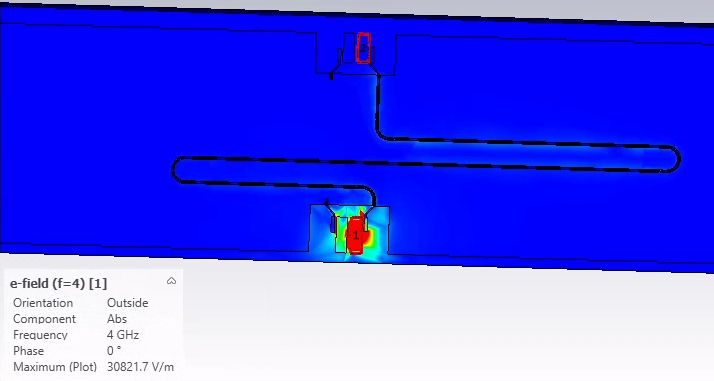
\includegraphics[width=\maxwidth,height=\maxheight,keepaspectratio]{images/cst-efield4.png}
\caption{Colored graph of the electric field intensity for a input frequency of 4GHz}
\label{cst-efield4}
\end{figure}

\begin{figure}[h]
\centering
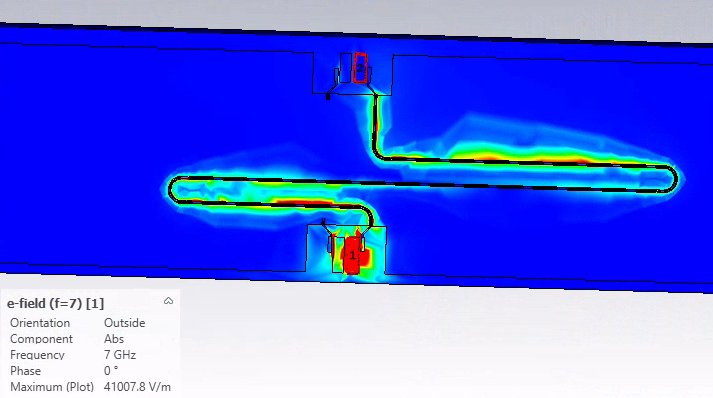
\includegraphics[width=\maxwidth,height=\maxheight,keepaspectratio]{images/cst-efield7.png}
\caption{Colored graph of the electric field intensity for a input frequency of 7GHz}
\label{cst-efield7}
\end{figure}

And finally we can get the resonance frequency by observing the graph of the output of the circuit in the frequency domain (figure \ref{cst-freq}). We can see the first resonance at around 6.5Ghz and another big one at 7.2-7.5Ghz followed by one at around 11Hz. 

The wire of the cavity has 9000$\mu$ of length and along with other specifications such as the thickness of the material deposited in the plate the calculated resonance frequency was 6.627GHz using a spreadsheet for circuit design available in the laboratory. Which is not far from the the first small resonance we see in figure \ref{cst-freq}. This resonance is used in the process of controlling the qubits in the quantum chip bring bringing them either in our out of resonance with the cavity for a iSWAP gate with the cavity for example.


\begin{figure}[h]
\centering
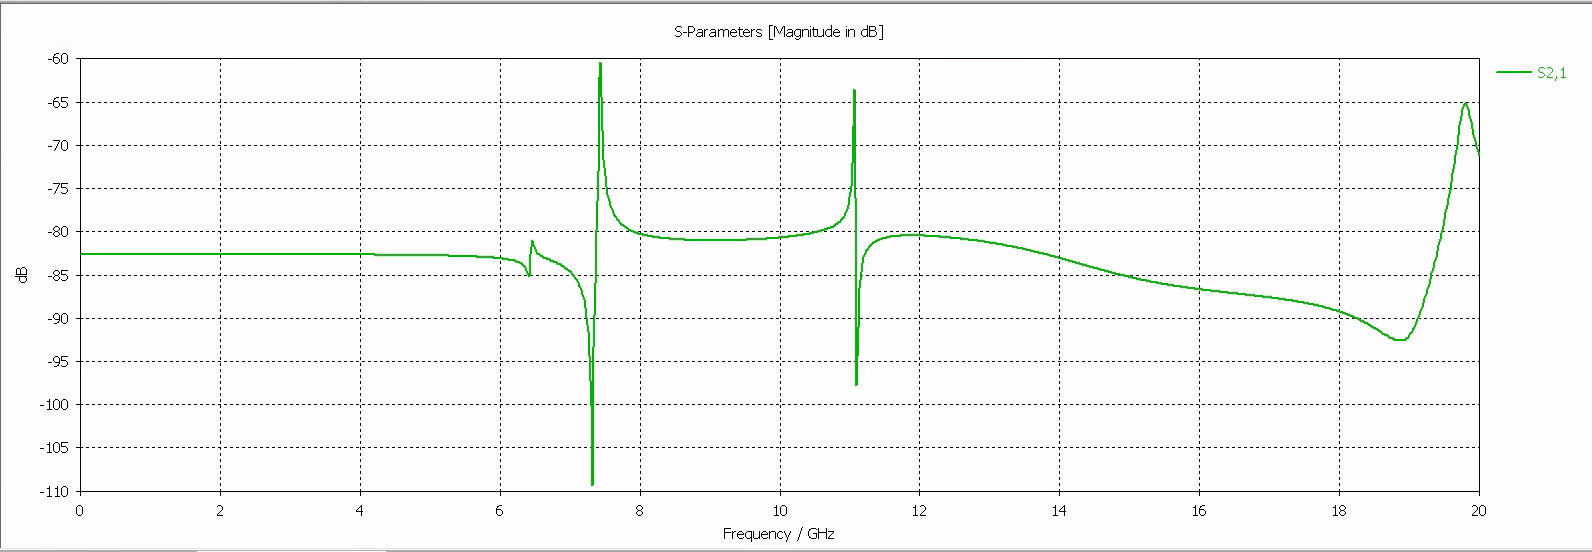
\includegraphics[width=\maxwidth,height=\maxheight,keepaspectratio]{images/cst-freq-domain.png}
\caption{Graph in the frequency domain of the amplitude of the signal between the two plates of different transmon qubits connected through a cavity.}
\label{cst-freq}
\end{figure}

\section{Conclusion}
The beginning of the project was more of a directed study of the basis of superconducting qubit. Going from the properties of the superconductor itself to the Josephson junction and the circuits using it. Here I was able to get a good grasp of the manner in which the superconductor qubits really work from the ground up. 

Different from my previous project of scientific initiation where the qubit was assumed to just work. I got to expand basic knowledge of quantum mechanics such as the quantum harmonic oscillator (cavity) with new notions such as non-linearity from the Josephson junction or driven cavities and resonators.

Then in the second part I used this knowledge to build simulations of the quantum circuits using their Hamiltonians. And do some more complex quantum computing operations with them such as a CNOT gate using two coupled qubits. For this part I had to develop better the knowledge of driving qubits with a signal. For which I used a different reference from the used in the beginning  \cite{2019krantz}. 

I also simulated the process of calibration of a coupling constant and the simulation of a measurement. This added to the feel of how it would be working with a real superconducting qubit in a laboratory. How it would be controlling it and getting output.

To finish the project I used a new tool by IBM called qiskit metal to design a superconducting chip. And then simulated part of it (the cavity between the qubits) in CST. Which was a bit difficult because CST requires one to know a lot of little tricks for it to work properly which requires experience. But I was still able to get a good simulation with the resonance frequency of the cavity visible.

Following the project I am going now beginning in August on an exchange program to France at Paristech ESPCI to get a double diploma in engineering. Hopefully to also continue my studies in the subject of superconducting quantum computing and get a Masters degree along with the bachelor diploma.

%%%%%%%%%%%%%%%%%%%%%%%%%%%%%%%%%%%%%%%%%%%%%%%%%
%\section{Continuation}

%Then we will do the Rabi measurements on the simulated system that describe the decay of the qubit to unusable states and thus its deterioration. Decay to the ground state from the excited state, relaxation ($T_1$) and the time for a state in superposition to go to a non-superposition state, dephasing ($T_2$).

%The third part is implementing the circuit in the IBM's tool called qiskit metal. Which has premade parts of a superconducting circuit that can be assembled simulated extracting data like the Hamiltonian of the system, dissipation and non-harmonicity.

%Finally the circuit developed in qiskit metal will be simulated in electromagnetic simulators by numerical methods using the Maxwell equations for discreet regions of spaced named meshes. Getting numerical solutions to the electrical and magnetic fields for systems with complex geometries such as this one.
\clearpage

\printbibliography

\end{document}
